%_____________________________________________________________________________________________
% LATEX Template: Department of Comp/IT BTech Project Reports
% Main Report
% Sun Apr 1 20:40:00 IST 2011
%
% Build with pdflatex:  latexmk -pdf coeptech_cse_report.tex
%_____________________________________________________________________________________________

\documentclass[a4paper,12pt,onecolumn]{report}

%_____________________________________________________________________________________________
% Inclusion of Required Packages
%_____________________________________________________________________________________________
\usepackage{graphicx}            % pdflatex: PDF/PNG/JPG figures (the template's [dvips]{graphics} needs latex+dvips)
\usepackage{color}
\usepackage{epsfig,float}
\usepackage[T1]{fontenc}
\usepackage{lmodern}             % scalable (Type 1) version of Computer Modern; avoids bitmap fonts
\usepackage{amsmath,amssymb}
\usepackage{booktabs,tabularx,multirow,longtable,array}
\usepackage{enumitem}
\usepackage{caption}
\usepackage{url}
\usepackage{algorithm}
\usepackage{algpseudocode}
\usepackage[expansion=false]{microtype}
\usepackage[hidelinks]{hyperref}
\setlength{\emergencystretch}{2em}
\captionsetup{font=small,labelfont=bf}
\setlist{itemsep=2pt,topsep=4pt}
\graphicspath{{figures/}{figures/screens/}}
%_____________________________________________________________________________________________
% Page Layout
%_____________________________________________________________________________________________

 \usepackage[left=2.5cm,top=2cm,right=2cm,bottom=2cm,bindingoffset=0.5cm]{geometry}

%\usepackage{geometry}
%\geometry{a4paper,left=35mm,right=20mm,top=20mm,bottom=20mm}
%\setlength{\textwidth}{6.5in}
%\setlength{\textheight}{10in}
%\setlength{\topmargin}{0.0in}
%\setlength{\oddsidemargin}{0.0in}			% Customisable
%\setlength{\headheight}{0.0in}
%\setlength{\headsep}{0.0in}
%\setlength{\topskip}{0.0in}
%_____________________________________________________________________________________________
% Font Definition
%_____________________________________________________________________________________________
\fontencoding{T1}		% Font specification : Times New Roman, Bold, Normal, 18
\fontfamily{lmr}		% Roman (Latin Modern = Computer Modern, scalable)
\fontseries{m}			% Medium
\fontshape{n}			% Upright
\fontsize{14pt}{5}
\linespread{1.5}		% Vertical spacing between lines
\selectfont			% Select the specified font

\newcommand{\figref}[1]{Fig.~\ref{#1}}
\newcommand{\tabref}[1]{Table~\ref{#1}}
%_____________________________________________________________________________________________
% Main report starts here
%_____________________________________________________________________________________________

\begin{document}	% Start of Report
%_____________________________________________________________________________________________
\pagenumbering{roman}
%_____________________________________________________________________________________________
% Title page: Specifies a custom-made title page
%_____________________________________________________________________________________________
\begin{titlepage}
\begin{center}
\LARGE{\bf{ML Model Drift Early-Warning System\\}}	% LARGE = 17.28
\vspace{10pt}
\Large{\bf{ B. Tech. Project Report\\}}		% Large = 14.40
\Large{\em{Submitted by\\}}
\begin{table}[htbp]
	\begin{center}
	\begin{tabular}{ l c c l }
	\Large\bf{Akshay Naphade} & & & \Large\bf{612303014} \\[0.3cm]
	\Large\bf{Rushikesh Kadepurkar} & & & \Large\bf{612303077} \\[0.3cm]
	\Large\bf{Parth Tatpuje} & & & \Large\bf{612303083} \\[0.3cm]
	\Large\bf{Vishnu Gurav} & & & \Large\bf{642403005} \\
	\end{tabular}
	\end{center}
	\end{table}

%names of advisors
\Large{Under the guidance of\\ }
\Large{\bf{Prof. Sunil Bhirud}\\}
\Large{COEP Technological University, Pune\\}
\vspace{8pt}
%coep logo added
\begin{figure}[h]
\centering

\includegraphics[width=5cm,height=5cm]{COEP_Tech_University_Logo.jpg}
\end{figure}

\large{\bf{DEPARTMENT OF COMPUTER SCIENCE \& ENGINEERING}}\\
\Large{\bf{COEP TECHNOLOGICAL UNIVERSITY\\ (COEP TECH), PUNE - 5}}
\vfill
\large{\bf{November 2026}}
\end{center}
\end{titlepage}

%_____________________________________________________________________________________________
% LATEX Template: Department of Comp/IT BTech Project Reports
% Certificate Page
% Sun Mar 27 10:25:35 IST 2011
%
% Note: UK English spellings used.
%_____________________________________________________________________________________________
\thispagestyle{empty}
\linespread{2}
\begin{center}			% LARGE = 18
	\large{\bf{DEPARTMENT OF COMPUTER SCIENCE \& ENGINEERING,\\
	      COEP TECHNOLOGICAL UNIVERSITY, PUNE - 5\\}}
\end{center}

\vspace{20pt}			% Vertical space between dept name and ``certi''

\begin{center}
	\Large{\bf{CERTIFICATE\\}}
\end{center}

\vspace{20pt}

\linespread{1.5}			% Double spacing between lines
\selectfont
\large{
Certified that this project titled, ``ML Model Drift Early-Warning System''
has been successfully completed by \\
\begin{table}[htbp]
	\begin{center}
	\begin{tabular}{ l c c l }
	\Large\bf{Akshay Naphade} & & & \Large\bf{612303014} \\ [0.3cm]
	\Large\bf{Rushikesh Kadepurkar} & & & \Large\bf{612303077} \\ [0.3cm]
	\Large\bf{Parth Tatpuje} & & & \Large\bf{612303081} \\ [0.3cm]
	\Large\bf{Vishnu Gurav} & & & \Large\bf{642303005} \\
	\end{tabular}
	\end{center}
	\end{table} \\
and is approved for the partial fulfillment of the requirements for the degree of
``B. Tech. Computer Engineering''.
}

\vspace{60pt}

\begin{center}		% Horizontal spacing used to keep the signatures in columns at the ends of
			% lines

SIGNATURE\hspace{\stretch{1}}SIGNATURE\\
\normalsize{\bf{Prof. Sunil Bhirud\hspace{\stretch{1}}Dr. Pradip Deshmukh\\
Project Guide\hspace{\stretch{1}}Head}\\
Department of CSE\hspace{\stretch{1}}Department of CSE\\
COEP Tech Pune,\hspace{\stretch{1}}COEP Tech Pune,\\
Shivajinagar, Pune - 5.\hspace{\stretch{1}}Shivajinagar, Pune - 5.}
\end{center}


%_____________________________________________________________________________________________
% LATEX Template: Department of Comp/IT BTech Project Reports
% Abstract of Report
% Sun Mar 27 10:34:00 IST 2011
%_____________________________________________________________________________________________
\newpage
\thispagestyle{empty}
\begin{center}
\Large \textbf{Plagiarism Report}
\end{center}
\vspace{1cm}
\noindent [On this page, add the scanned copy of the plagiarism percentage page signed by the Project Guide.]

\newpage
\begin{center}
\Large \textbf{Acknowledgement}
\end{center}
\addcontentsline{toc}{chapter}{Acknowledgement}

We thank our guide, Prof.\ Sunil Bhirud, for his guidance and feedback throughout the project. We thank Dr.\ Pradip Deshmukh, Head of the Department of Computer Science and Engineering, and the faculty and staff of COEP Technological University, Pune, for providing the facilities and support needed to complete this work.

We used open-source tools and public datasets from OpenML, scikit-learn, NumPy, SciPy, pandas, matplotlib and Streamlit, and we thank their maintainers.

\vspace{1cm}
\begin{flushright}
Akshay Naphade\\
Rushikesh Kadepurkar\\
Parth Tatpuje\\
Vishnu Gurav
\end{flushright}

\newpage
\begin{center}
\Large \textbf{Abstract}
\end{center}
\addcontentsline{toc}{chapter}{Abstract}

Machine learning models deployed in production lose accuracy when the data they see drifts away from the data they were trained on. In many applications, such as credit, fraud or churn prediction, the true labels that would reveal this loss arrive days or weeks later. Drift detectors offer earlier, label-free signals, but most input shifts do not harm a given model, and alert thresholds tuned on one dataset often do not hold on another.

This project builds and evaluates an \emph{ML Model Drift Early-Warning System} that tries to warn when the model's accuracy is about to fall, before delayed labels can show it. We developed a benchmark that re-samples real tabular data from OpenML so that inputs drift from a known batch while every row keeps its true label; this lets us measure harm instead of assuming it. The system was developed over ten versions. Versions v1--v5 were exploratory studies on synthetic and natural data streams. Versions v6--v10 were pre-registered: every hypothesis, pass rule and alert threshold was frozen and fingerprinted in code before the confirmation data were downloaded, and each verdict was computed once by a script.

The first pre-registered design (v6), a learned risk calibrator over raw drift scores, failed all five of its hypotheses, because thresholds in dataset-specific units did not transfer: false alerts on unseen datasets ranged from 1.2 to 44.6 per 100 clean batches against a budget of 5. Expressing every signal relative to the stream's own burn-in period fixed this on benchmark streams. The resulting \emph{drift-watch} tier (v7) warned before the accuracy drop on 87\% of harmful gradual shifts on six fresh datasets, a median of six batches ahead, at 4.4 false alerts per 100 clean batches; it failed on natural streams, where drift was already under way when monitoring began. A second \emph{harm} tier (v8) estimates the model's accuracy from an importance-weighted labeled reference set. On five further fresh datasets it cut alarms on harmless shifts from 97\% to 34\% and separated harmful from harmless shifts with an AUROC of 0.78 (95\% CI 0.70--0.86), just below the pre-registered target of 0.80 but clearly above confidence-based baselines (0.56--0.59) on the same data. On a later set of six datasets the same rule exceeded the false-alert budget (12.7 per 100). Two follow-up experiments, nonlinear harm estimators (v9) and stricter alerting rules (v10), did not improve on it and were not adopted.

The project delivers the benchmark and monitoring code, frozen configurations and verdict scripts, a Streamlit dashboard that replays monitored streams batch by batch with delayed labels, a continuous-integration pipeline, and a research paper.

\vspace{0.5cm}
\noindent\textbf{Keywords:} concept drift, dataset shift, model monitoring, delayed labels, performance estimation, importance weighting, pre-registration, MLOps
%_____________________________________________________________________________________________
	% Abstract: Independently typeset in file abstract.tex

\tableofcontents		% LATEX needs to run 2-3 times over source to get this correct

\listoftables
\addcontentsline{toc}{chapter}{List of Tables}

\listoffigures
\addcontentsline{toc}{chapter}{List of Figures}

\chapter*{List of Symbols and Abbreviations}
\addcontentsline{toc}{chapter}{List of Symbols and Abbreviations}

\begin{longtable}{@{}p{3.2cm}p{11.8cm}@{}}
\toprule
\textbf{Symbol} & \textbf{Meaning} \\
\midrule
\endhead
$f$ & Frozen (monitored) binary classifier \\
$R$ & Labeled reference set (2000 rows) on which $f$ was fitted \\
$B_t$ & Batch number $t$ of the monitored stream (300 rows) \\
$L$ & Label delay in batches; labels of batch $b$ are usable from batch $b+\max(L,1)$ \\
$s$ & Batch at which the controlled intervention (shift) starts \\
$e$ & Batch at which the accuracy event starts \\
$\lambda(t)$, $\lambda_{max}$ & Shift strength at batch $t$ and its maximum (1.5) \\
$z_j$ & Feature $j$ standardized with reference statistics \\
$\sigma$ & Random shift direction, $\pm 1$ \\
$x_t$ & Value of a monitoring signal at batch $t$ \\
$\mathrm{med}$, $\mathrm{MAD}$ & Median and median absolute deviation \\
$g_t$ & Domain classifier separating reference rows from batch $B_t$ \\
$\rho_i$, $w_i$ & Odds of reference row $i$ under $g_t$, and its capped importance weight \\
$c_i$ & Correctness of $f$ on reference row $i$ ($1$ if correct) \\
$\hat a_t$ & Label-free (importance-weighted) estimate of the accuracy of $f$ on $B_t$ \\
$h_t$ & Harm score: estimated accuracy drop since the burn-in \\
T1, T2, T3 & Warning tiers: predictive, pre-confirmation, confirmed \\
FA & False alerts per 100 clean batches \\
\midrule
AUROC & Area under the receiver operating characteristic curve \\
CBPE & Confidence-based performance estimation \\
CI & Confidence interval (95\% bootstrap unless stated) or continuous integration \\
DEWS & Drift Early-Warning System (the original project prototype) \\
IW & Importance weighting \\
KS & Kolmogorov--Smirnov statistic \\
MMD & Maximum mean discrepancy \\
PSI & Population stability index \\
RWS & Relevance-weighted shift \\
kNN & $k$-nearest neighbors \\
\bottomrule
\end{longtable}


\newpage
\pagenumbering{arabic}	% Change to Arabic numbers for main chapters.

%_____________________________________________________________________________________________
% Chapter 1: Introduction
%_____________________________________________________________________________________________

\chapter{Introduction}
\label{ch:intro}

\section{Background}
A machine learning classifier is trained once, on data collected in the past, and is then deployed to make predictions on new data for months or years. The world that generates that data keeps changing: customers change their behavior, sensors age, upstream software changes how a feature is computed, and new kinds of cases appear. When the distribution of the incoming data moves away from the training distribution, the model may start making more mistakes. This phenomenon is known as \emph{dataset shift} or \emph{concept drift}~\cite{gama2014survey,quinonero2009shift}.

The obvious way to notice a drop in accuracy is to compare the model's predictions with the true outcomes. In many real applications, however, the true outcome (the \emph{label}) arrives only after a long delay. Whether a loan defaults is known after months; whether a transaction was fraudulent is known after a chargeback; whether a customer churned is known at the end of a billing cycle. During this delay the model keeps making decisions, and a silent degradation can cause real damage before anyone sees it.

Monitoring tools therefore watch signals that need no labels, such as feature distributions, model confidence and the mix of predicted classes~\cite{sculley2015debt,breck2017mltest}. These signals are available at once, but they have two problems:
\begin{enumerate}
\item \textbf{Most shifts are harmless.} A change in the inputs does not necessarily change the model's accuracy~\cite{rabanser2019failing}. A drift detector that alarms on every change produces many alarms that do not matter, and operators learn to ignore it.
\item \textbf{Thresholds do not transfer.} An alert threshold is normally tuned on historical data from one application. Whether the same threshold still means the same thing on another dataset, or even on the same dataset next year, is rarely tested.
\end{enumerate}

\section{Motivation}
The project started from an existing prototype, the \emph{Drift Early-Warning System} (DEWS). It combined several drift statistics (Kolmogorov--Smirnov tests, the population stability index, an embedding-based maximum mean discrepancy and a confidence component) into a single fused drift score, compared it with an adaptive threshold, and forecast when the score would cross the threshold. The prototype also contained a FastAPI service, a SQLite store, and a large infrastructure stack (Kafka, Celery, Redis and Grafana).

Our first careful evaluation of this prototype was negative. On held-out controlled episodes its learned risk calibrator detected 0 of 20 harmful events, and the fused drift score detected some events only after the accuracy had already dropped (Section~\ref{sec:v1}). The infrastructure was complete, but nothing showed that the warnings came early or that they matched real accuracy loss.

We therefore stopped adding components and narrowed the project to one question, tested so that a negative answer would show up as clearly as a positive one.

\section{Problem Statement}
\begin{quote}
Given a frozen binary classifier, a stream of unlabeled batches, and true labels that arrive only after a delay of $L$ batches, build a monitor that warns about a sustained loss of accuracy (a) before the accuracy actually drops, and (b) before the delayed labels could confirm the drop, while raising at most 5 false alerts per 100 batches of unchanged data, and while separating shifts that harm the model from shifts that do not.
\end{quote}
The precise definitions of a degradation event, the warning tiers and the false-alert budget are given in Chapter~\ref{ch:problem}.

\section{Objectives}
\begin{enumerate}
\item Build a realistic benchmark on real tabular datasets in which input shifts start at a known batch while every row keeps its true label, so that whether a shift harmed the model can be measured rather than assumed.
\item Design label-free monitoring signals and an alerting scheme that warn early about harmful drift within a fixed false-alert budget.
\item Separate harmful from harmless shifts without using the labels of the monitored batches.
\item Evaluate every claim with pre-registered hypotheses, frozen thresholds and one-time runs on datasets that were never used during design, and report failures as clearly as successes.
\item Deliver a working, reproducible product: the monitoring library, experiment scripts, a dashboard that replays monitored streams, automated tests and continuous integration, and a research paper.
\end{enumerate}

\section{Scope}
\textbf{In scope.} One frozen binary classifier on tabular data (logistic regression as the primary model, gradient boosting as a robustness check); batches of 300 rows; label delays of 0, 2, 5 and 10 batches; controlled covariate shifts and label changes built from real data; natural row-order streams as a reality check; and an offline replay dashboard.

\textbf{Out of scope.} Automated retraining, distributed stream processing, production throughput and failover, image or text models, and claims about arbitrary concept drift. The Kafka, Celery, Redis and Grafana stack of the original prototype was removed from the repository because it did not contribute to the research question.

\section{Contributions}
\begin{enumerate}
\item A re-sampling benchmark that turns real OpenML datasets into monitored streams with gradual, abrupt and irrelevant-feature shifts and label changes with a known onset, in which harm is measured from true labels.
\item Evidence that drift thresholds expressed in raw, dataset-specific units do not transfer across datasets, and that expressing every signal relative to a stream's own burn-in period largely fixes this: the resulting drift watch held its false-alert budget on unseen benchmark data, though not on natural streams.
\item A label-free harm tier based on importance-weighted reference accuracy, which cuts alarms on harmless shifts and separates harm better than confidence-based estimates on the same data.
\item A complete record of pre-registered negative results: a failed first design, a failed second tier, a benchmark gate that failed, and two follow-up attempts that were not adopted.
\item A reproducible software product: library, frozen configurations, verdict scripts, dashboard, 85 unit tests, continuous integration, and a research paper prepared for IEEE CONECCT and arXiv.
\end{enumerate}

\section{Organization of the Report}
Chapter~\ref{ch:lit} surveys related work on drift detection, label-free performance estimation, delayed labels and pre-registration. Chapter~\ref{ch:problem} defines the problem formally and lists the requirements. Chapter~\ref{ch:design} presents the system architecture, the two-tier monitor, the benchmark and the evaluation protocol. Chapter~\ref{ch:impl} describes the implementation, including the exploratory versions v1--v5, the code structure, the dashboard and the testing infrastructure. Chapter~\ref{ch:results} reports and discusses the results of the pre-registered experiments v6--v10, the ablations and the post hoc analyses. Chapter~\ref{ch:conclusion} concludes and outlines future work. The appendices list every pre-registered hypothesis, the datasets used, and the commands needed to reproduce the results.
	% Introduction
%_____________________________________________________________________________________________
% Chapter 2: Literature Survey
%_____________________________________________________________________________________________

\chapter{Literature Survey}
\label{ch:lit}

We review concept drift and dataset shift, drift detection, label-free accuracy estimation, delayed labels and pre-registration.

\section{Concept Drift and Dataset Shift}
Gama et al.~\cite{gama2014survey} and Lu et al.~\cite{lu2019review} survey concept drift: changes over time in the joint distribution $P(X, Y)$ of inputs $X$ and labels $Y$. It is useful to separate two cases~\cite{quinonero2009shift}:
\begin{itemize}
\item \textbf{Covariate shift}: $P(X)$ changes while $P(Y\mid X)$ stays the same. The model's decision rule is still correct where it was correct, but the data may move into regions where the model was weak.
\item \textbf{Concept shift}: $P(Y\mid X)$ changes, so the same input now has a different correct label. No input-only signal can see this; only labels reveal it.
\end{itemize}
Label shift, where $P(Y)$ changes and $P(X\mid Y)$ stays the same, is treated by Lipton et al.~\cite{lipton2018labelshift}.

\section{Drift Detection}
\subsection{Detectors that need labels}
Classical detectors monitor the error stream of a model. DDM~\cite{gama2004ddm} signals a warning and then a drift when the error rate rises significantly above its historical minimum. ADWIN~\cite{bifet2007adwin} keeps an adaptive window and cuts it when two sub-windows have significantly different means. Sequential tests such as CUSUM~\cite{page1954cusum} accumulate evidence of a persistent change. All of these need the label of each prediction, so with delayed labels they react late by construction.

\subsection{Label-free detectors}
Label-free detection compares the distribution of the current inputs with a reference sample. Common statistics are the two-sample Kolmogorov--Smirnov (KS) test per feature~\cite{massey1951ks}, the population stability index (PSI) used in credit scoring, divergences between histograms, and the kernel maximum mean discrepancy (MMD)~\cite{gretton2012mmd}. Rabanser et al.~\cite{rabanser2019failing} compared such detectors systematically and noted an important limitation: a detected shift need not reduce accuracy. Open-source monitoring tools such as Evidently~\cite{evidently} and NannyML~\cite{nannyml_cbpe} package these statistics for practitioners.

\section{Label-Free Performance Estimation}
A second line of work estimates the model's accuracy directly, without labels:
\begin{itemize}
\item \textbf{Confidence-based estimation (CBPE)}~\cite{nannyml_cbpe} uses the model's predicted probabilities as the expected accuracy. It is exact only if the model is calibrated on the new data.
\item \textbf{Average thresholded confidence (ATC)}~\cite{garg2022atc} learns a confidence threshold on source data and predicts the target accuracy as the share of target examples above it.
\item \textbf{Difference of confidences (DoC)}~\cite{guillory2021doc} regresses the accuracy change on the change in average confidence.
\item \textbf{Disagreement}~\cite{jiang2022disagreement}: the rate at which two independently trained models disagree tracks their error rate under certain conditions.
\item \textbf{Importance weighting}~\cite{shimodaira2000,sugiyama2007iwcv}: under covariate shift, reweighting labeled source examples by the density ratio $p_{target}(x)/p_{source}(x)$ gives an unbiased estimate of any target expectation, including accuracy. The density ratio can be estimated with a probabilistic classifier that separates source from target samples.
\end{itemize}
Our harm tier (Section~\ref{sec:harm}) uses importance weighting with a logistic domain classifier, applied to the model's correctness on the labeled reference set.

\section{Delayed Labels}
Learning and evaluation with delayed or partially missing labels are studied by Grzenda et al.~\cite{grzenda2020delayed} and Umer and Polikar~\cite{umer2020evl}. In the monitoring setting the key point is causality: at batch $t$, only the labels of batches $b \le t-\max(L,1)$ may be used. Any evaluation that ignores this leaks future information and overstates how early a monitor can warn. Our replay protocol enforces this rule and tests it (Section~\ref{sec:tests}).

\section{Pre-Registration and Reproducibility}
Pre-registration means fixing hypotheses, analysis methods and success criteria before seeing the data that will judge them~\cite{nosek2018prereg}. It reduces the freedom to choose, after the fact, the analysis that looks best. Van Miltenburg et al.~\cite{vanmiltenburg2021prereg} discuss pre-registration for machine learning and natural language processing research. Sculley et al.~\cite{sculley2015debt} and Breck et al.~\cite{breck2017mltest} argue that production ML systems need explicit, testable monitoring. We apply pre-registration to the evaluation of a monitoring system, including its alert thresholds, and we use public datasets from OpenML~\cite{vanschoren2014openml} so that every result can be reproduced.

\section{Summary and Research Gap}
\tabref{tab:lit} summarises the main families of methods.

\begin{table}[H]
\caption{Families of drift-monitoring methods and their limits in the delayed-label setting.}
\label{tab:lit}
\centering
\small
\begin{tabularx}{\textwidth}{@{}p{3.4cm}p{3.2cm}X@{}}
\toprule
Family & Examples & Limitation for early warning with delayed labels \\
\midrule
Error-stream detectors & DDM, ADWIN, CUSUM & Need labels; with delay $L$ they react at least $L$ batches late \\
Input-distribution tests & KS, PSI, MMD, fused scores & Detect any change, harmful or not; thresholds in dataset-specific units \\
Confidence-based estimators & CBPE, ATC, DoC & Assume calibration on new data; can stay confident while wrong \\
Disagreement & auxiliary models & Moves with any shift that the auxiliary models notice \\
Importance weighting & density-ratio reweighting & Valid only under covariate shift; needs a labeled reference sample \\
\bottomrule
\end{tabularx}
\end{table}

Three things are missing from this work:
\begin{enumerate}
\item Most evaluations report whether drift is detected, not whether a warning comes \emph{before} the accuracy drop or \emph{before} delayed labels could reveal it.
\item Alert thresholds are rarely tested on datasets other than the ones they were chosen on.
\item Few studies measure, on real data with known ground truth, how often a drift alarm corresponds to actual harm.
\end{enumerate}
The project addresses these gaps with a benchmark in which harm is measured, warning tiers defined relative to label arrival, and pre-registered confirmation on datasets never used during design.
	% Literature survey
%_____________________________________________________________________________________________
% Chapter 3: Problem Definition and Requirements
%_____________________________________________________________________________________________

\chapter{Problem Definition and Requirements}
\label{ch:problem}

\section{Formal Problem Setting}
A frozen binary classifier $f$ is trained on a labeled reference set $R$ and then scores a stream of batches $B_0, B_1, B_2, \dots$ of 300 rows each. The monitor sees the rows of every batch and the predictions of $f$ immediately. The true labels of batch $b$ become usable at batch $b+\max(L,1)$, where $L$ is the label delay (primary setting $L=5$). The first 8 batches after deployment form a \emph{burn-in} period during which no alerts are raised; the monitor uses them to learn what normal looks like for this stream.

\subsection{Degradation event}
The baseline accuracy is the mean accuracy of $f$ on batches 0--4. A \emph{degradation event} begins at the first of two consecutive batches whose accuracy is at least 5 percentage points below the baseline. Requiring two consecutive batches avoids calling a single noisy batch an event.

\subsection{Episodes and outcomes}
An \emph{episode} is one monitored stream of 45 batches. In controlled episodes an intervention starts at a known batch $s$. Each shift episode is then labelled from the true accuracy:
\begin{itemize}
\item \textbf{Harmful}: an event starts at or after $s$;
\item \textbf{Harmless}: no event occurs;
\item \textbf{Spurious}: an event starts before $s$ (or occurs in a clean episode); spurious episodes are excluded from the main hypotheses and their number is reported.
\end{itemize}

\subsection{Warning tiers}
For an intervention at batch $s$ and an event at batch $e$ we distinguish three tiers (\figref{fig:tiers}):
\begin{itemize}
\item \textbf{T1, predictive warning}: an alert in $[s, e)$, before the accuracy actually drops. The \emph{lead time} is $e$ minus the first such alert.
\item \textbf{T2, pre-confirmation warning}: an alert in $[s, e+1+\max(L,1))$, before delayed labels could confirm the event. In practice T2 matters most, because it measures what the monitor adds over waiting for labels.
\item \textbf{T3, confirmed}: the first alert at or after confirmation; by then the labels already show the drop.
\end{itemize}

\begin{figure}[H]
\centering
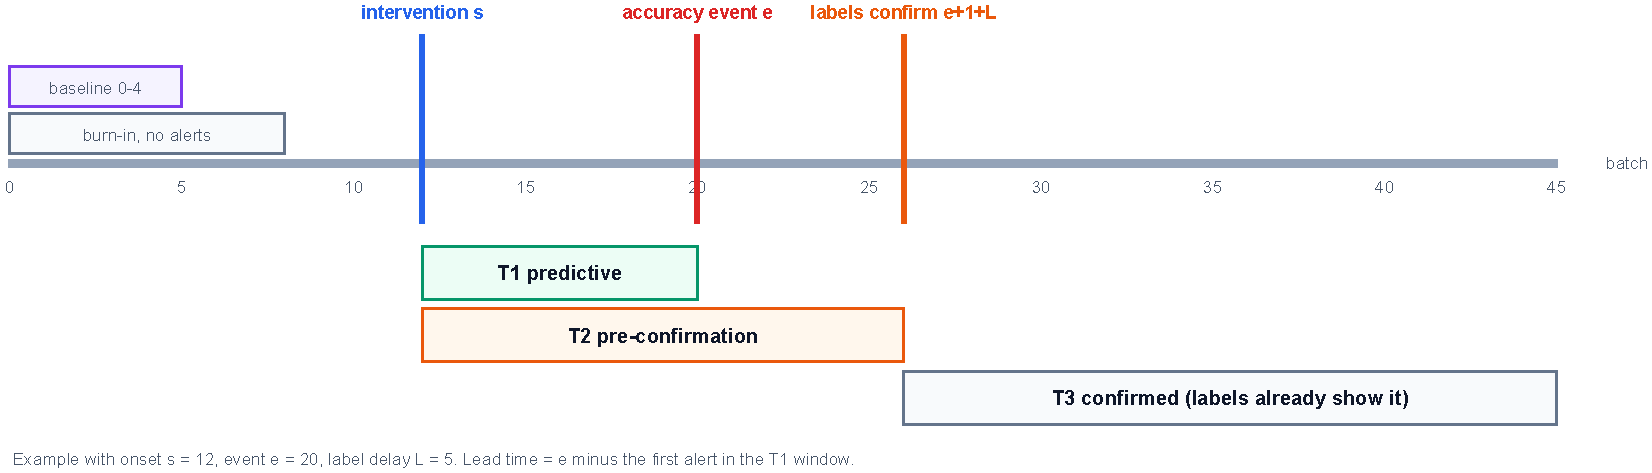
\includegraphics[width=\textwidth]{fig_warning_tiers.pdf}
\caption{Warning tiers on the batch axis, for onset $s=12$, event $e=20$ and label delay $L=5$. T1 ends when accuracy drops; T2 ends when delayed labels could confirm the drop.}
\label{fig:tiers}
\end{figure}

\subsection{False alerts}
\emph{Clean batches} are all batches of unshifted (clean) episodes and the pre-intervention batches of every other episode. The \emph{false-alert rate} is the number of alerts on clean batches per 100 clean batches, with a budget of \textbf{5}. For harmless shifts, which never cause an event, we report the \emph{harmless-alarm share}: the share of harmless episodes with any alert after onset.

\subsection{Separation of harm}
To measure whether a score separates harmful from harmless shifts, we take its mean over the first 3 batches after onset in each shift episode and compute the area under the ROC curve (AUROC) between harmful and harmless episodes. An AUROC of 0.5 means no separation; 1.0 means perfect separation.

\section{Functional Requirements}
\begin{enumerate}[label=FR\arabic*.]
\item \textbf{Stream construction.} Build monitored episodes from any binary tabular OpenML dataset: reference set, pool, 45 batches, controlled shifts with a known onset, and true labels for every row.
\item \textbf{Signal extraction.} For every batch, compute label-free signals: per-feature drift statistics, the fused DEWS drift score, relevance-weighted shift, positive-rate shift, confidence, entropy, and disagreement with auxiliary models.
\item \textbf{Delayed labels.} Release the labels of batch $b$ only at batch $b+\max(L,1)$; never let a score at batch $t$ use a label that has not matured.
\item \textbf{Drift watch.} Normalise every signal against the stream's burn-in and raise a WATCH alert when the largest normalised signal exceeds the frozen threshold.
\item \textbf{Harm tier.} Estimate the model's current accuracy from the labeled reference set by importance weighting and raise a HARM alert when the estimated drop exceeds the frozen threshold.
\item \textbf{Confirmation.} When delayed labels arrive, confirm or clear the warning with the event rule.
\item \textbf{Evaluation.} Compute T1, T2, T3, lead times, false-alert rates, harmless-alarm shares and AUROC with bootstrap confidence intervals.
\item \textbf{Pre-registration.} Freeze thresholds and rules in versioned configuration files with SHA-256 fingerprints, and refuse to run a confirmation if a fingerprint does not match.
\item \textbf{Verdicts.} Apply the frozen pass rules mechanically and write a verdict file and report.
\item \textbf{Dashboard.} Replay a saved episode batch by batch with a chosen label delay, show both tiers and the delayed labels, explain which signals moved, and show all verdicts and ablations.
\end{enumerate}

\section{Non-Functional Requirements}
\begin{enumerate}[label=NFR\arabic*.]
\item \textbf{Causality.} No score may use future labels or event outcomes; this is enforced in code and covered by unit tests.
\item \textbf{Reproducibility.} Every episode is generated from a recorded seed; all models use fixed random states; bootstrap intervals use fixed generator seeds; a single command rebuilds and verifies the verdicts.
\item \textbf{Honesty of evaluation.} Thresholds are chosen on development data only; confirmation data are downloaded only after the design is frozen; each confirmation is run once.
\item \textbf{Performance.} Monitoring a batch must take well under a second on a laptop; the earlier replay pipeline measured about 0.08 seconds per batch.
\item \textbf{Maintainability.} Code is linted (Ruff), unit-tested (pytest) and checked by continuous integration on Python 3.10, 3.11 and 3.12.
\item \textbf{Usability.} The dashboard must be understandable to a non-specialist examiner in a short demonstration.
\end{enumerate}

\section{Hardware and Software Requirements}
\begin{table}[H]
\caption{Hardware and software used.}
\label{tab:env}
\centering
\small
\begin{tabularx}{\textwidth}{@{}p{3.5cm}X@{}}
\toprule
Item & Specification \\
\midrule
Hardware & Laptop, Intel Core i7-12650H (10 cores, 16 threads), 16 GB RAM; no GPU needed \\
Operating system & Windows 11 (development); Ubuntu (continuous integration) \\
Language & Python 3.10--3.12 (development on 3.12) \\
Core libraries & NumPy 2.5.4, SciPy, pandas 2.3, scikit-learn 1.7.2, statsmodels, matplotlib \\
Dashboard & Streamlit 1.57+, Altair \\
Testing and CI & pytest 8, Ruff 0.17.4, GitHub Actions \\
Data source & OpenML~\cite{vanschoren2014openml}, fetched with scikit-learn \\
Documents & \LaTeX\ (IEEEtran for the paper, this template for the report), draw.io for diagrams \\
Legacy (optional) & FastAPI, uvicorn, MLflow, PostgreSQL drivers, in a separate environment \\
\bottomrule
\end{tabularx}
\end{table}

\section{Users and Use Cases}
Two kinds of users interact with the system (\figref{fig:usecases}). An \emph{ML engineer} uses the monitor and the dashboard to see whether a deployed model is drifting and whether the drift is likely to hurt it. A \emph{researcher or examiner} reads the verdicts, reproduces them, and runs new pre-registered experiments. OpenML acts as an external system that supplies datasets.

\begin{figure}[H]
\centering
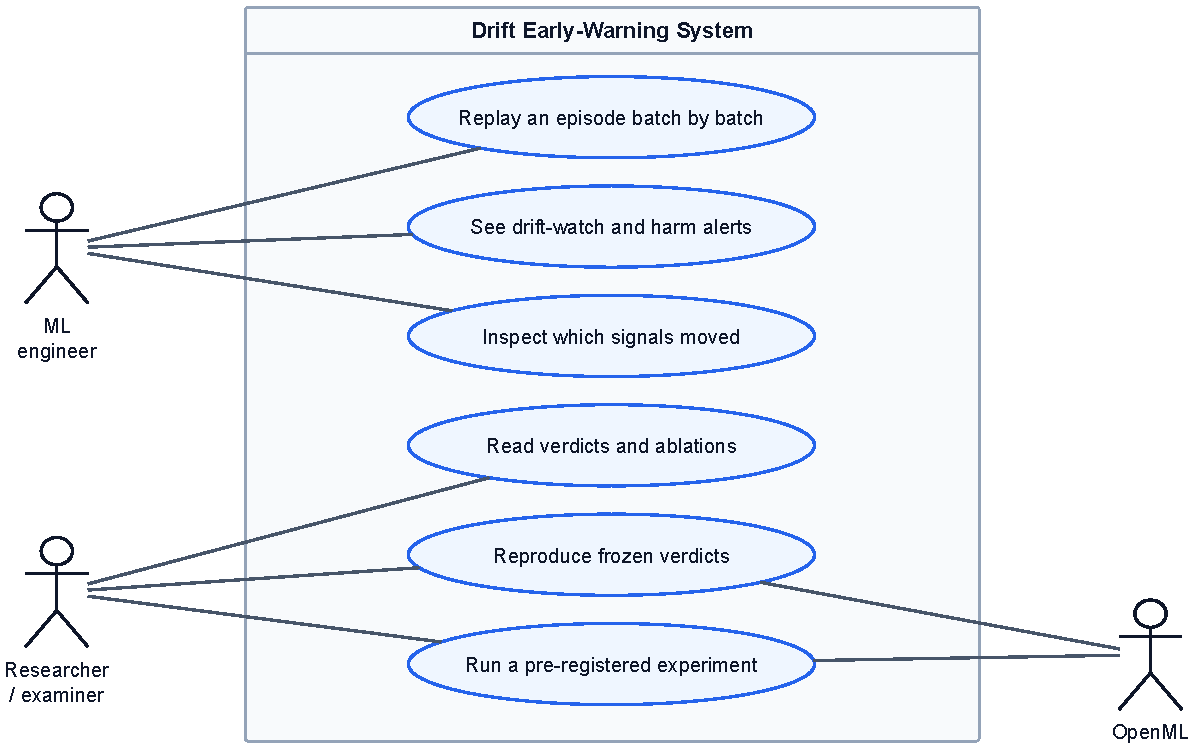
\includegraphics[width=0.8\textwidth]{fig_usecases.pdf}
\caption{Use-case diagram of the Drift Early-Warning System.}
\label{fig:usecases}
\end{figure}
	% Problem definition and requirements
%_____________________________________________________________________________________________
% Chapter 4: System Design
%_____________________________________________________________________________________________

\chapter{System Design}
\label{ch:design}

This chapter describes the design of the final system: its architecture, the benchmark that produces monitored streams with known ground truth, the label-free signals, the two warning tiers, and the protocol used to evaluate them. The history of how the design was reached is given in Chapter~\ref{ch:impl}.

\section{System Architecture}
\figref{fig:arch} shows the architecture as five layers.
\begin{itemize}
\item \textbf{Data.} Public tabular datasets from OpenML feed a benchmark generator, which builds monitored streams with a known intervention batch. Natural row-order streams are used as a reality check.
\item \textbf{Model.} A frozen classifier $f$ is fitted once on a labeled reference set $R$. Each incoming batch $B_t$ is scored by $f$; its labels stay hidden.
\item \textbf{Signals.} Label-free signals are computed per batch: input-shift statistics and model-behaviour statistics.
\item \textbf{Monitor.} Two tiers turn the signals into alerts: a \emph{drift watch} that is sensitive to any drift, and a \emph{harm tier} that estimates whether the drift is lowering accuracy.
\item \textbf{Outputs.} Alerts are confirmed or cleared when delayed labels arrive. Evaluation scripts compute the warning tiers and apply the pre-registered pass rules; the dashboard, paper and this report are generated from the saved results.
\end{itemize}

\begin{figure}[H]
\centering
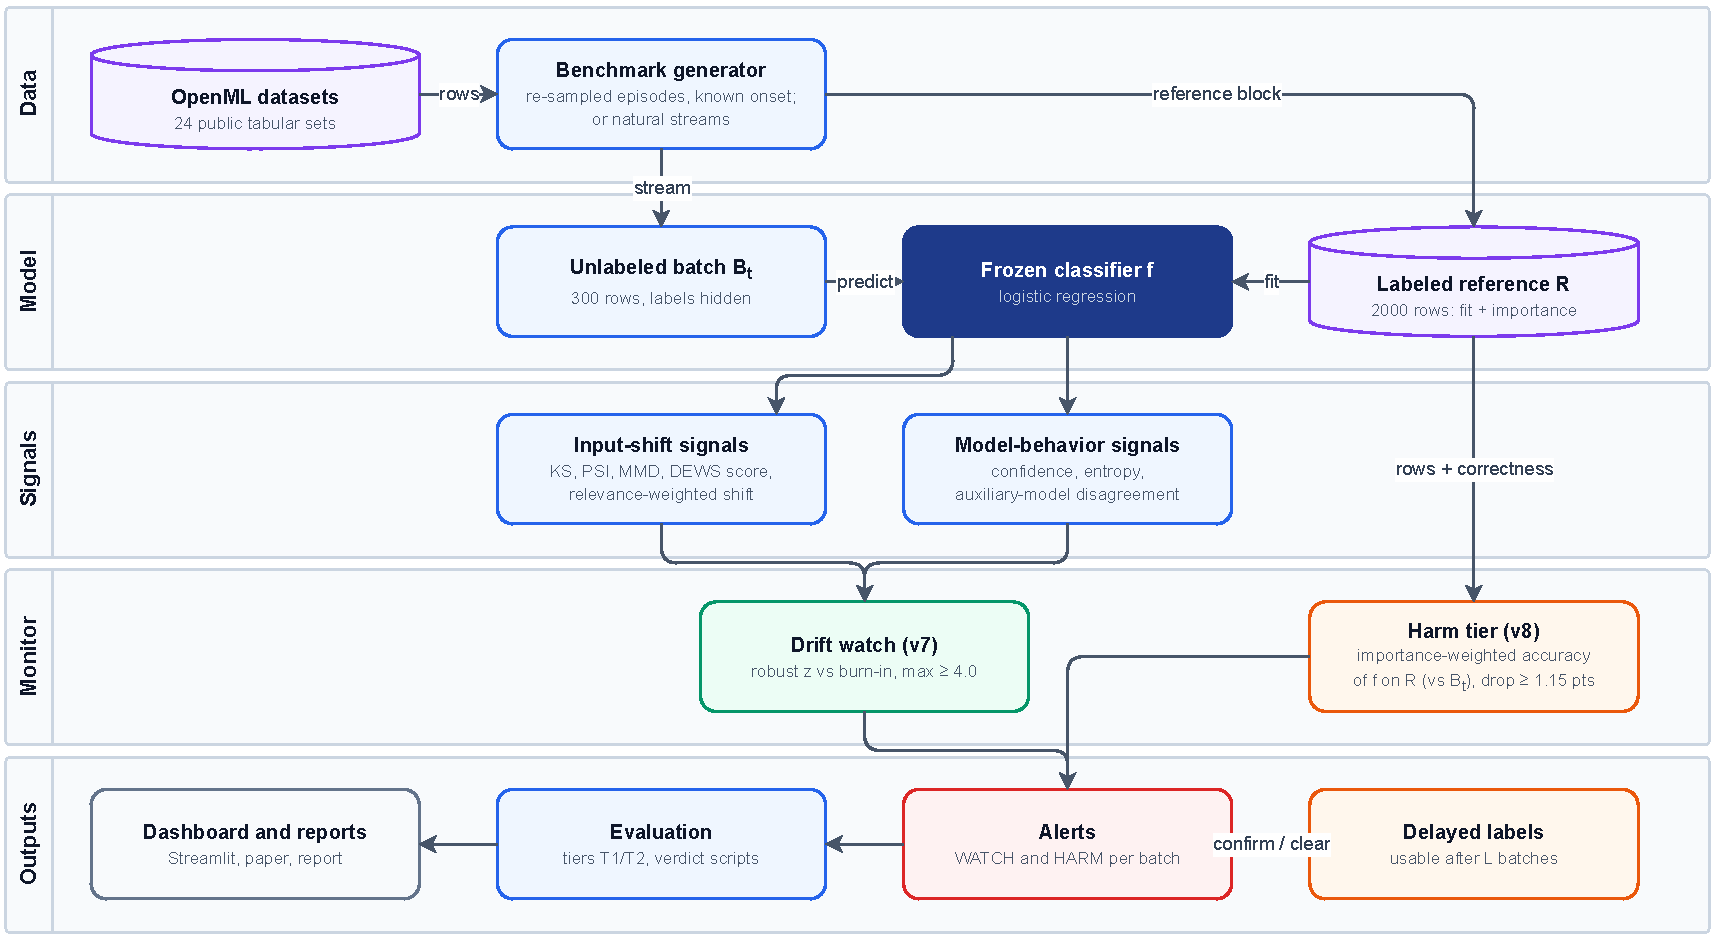
\includegraphics[width=\textwidth]{fig_architecture.pdf}
\caption{Layered architecture of the ML Model Drift Early-Warning System.}
\label{fig:arch}
\end{figure}

\section{Benchmark Design}
\label{sec:benchmark}
Evaluating an early-warning system needs ground truth: we must know when a shift started and whether it actually hurt the model. Synthetic generators provide this but are unrealistic (Section~\ref{sec:v2}); natural streams are realistic but have no known onset. The benchmark combines the two by \emph{re-sampling real rows}.

Each episode draws a contiguous block of a dataset (\figref{fig:episode}):
\begin{itemize}
\item a \textbf{reference} of 2000 rows: $f$ is fitted on the first 1500, and the last 500 are held out to compute $f$'s permutation feature importance;
\item a \textbf{pool} of the next 20,000 rows. Because reference and pool come from the same period, an unshifted stream has no built-in drift.
\end{itemize}
The stream has 45 batches of 300 rows sampled with replacement from the pool; \emph{every row keeps its true label}, so the true accuracy of $f$ on every batch is known. From an onset batch $s \in [10,16]$:
\begin{itemize}
\item \textbf{Gradual or abrupt shift}: rows are sampled with weights proportional to $\exp(\lambda(t)\,\sigma\,z_j)$, where $z_j$ is a standardised feature, $\sigma=\pm 1$ a random direction, and $\lambda$ ramps linearly to 1.5 over 15 batches (gradual) or jumps to 1.5 (abrupt). The feature $j$ is drawn from the more important or the less important half of features with equal probability, so that some shifts are designed to be irrelevant.
\item \textbf{Label change}: labels are flipped with a probability that ramps to 0.3 for rows with $z_k>0$, a change in $P(Y\mid X)$ that input-only signals cannot see.
\item \textbf{Clean}: uniform sampling.
\end{itemize}
Each dataset contributes 10 clean, 30 gradual, 15 abrupt and 10 label-change episodes (65 episodes). Algorithm~\ref{alg:episode} summarises the construction.

\begin{figure}[H]
\centering
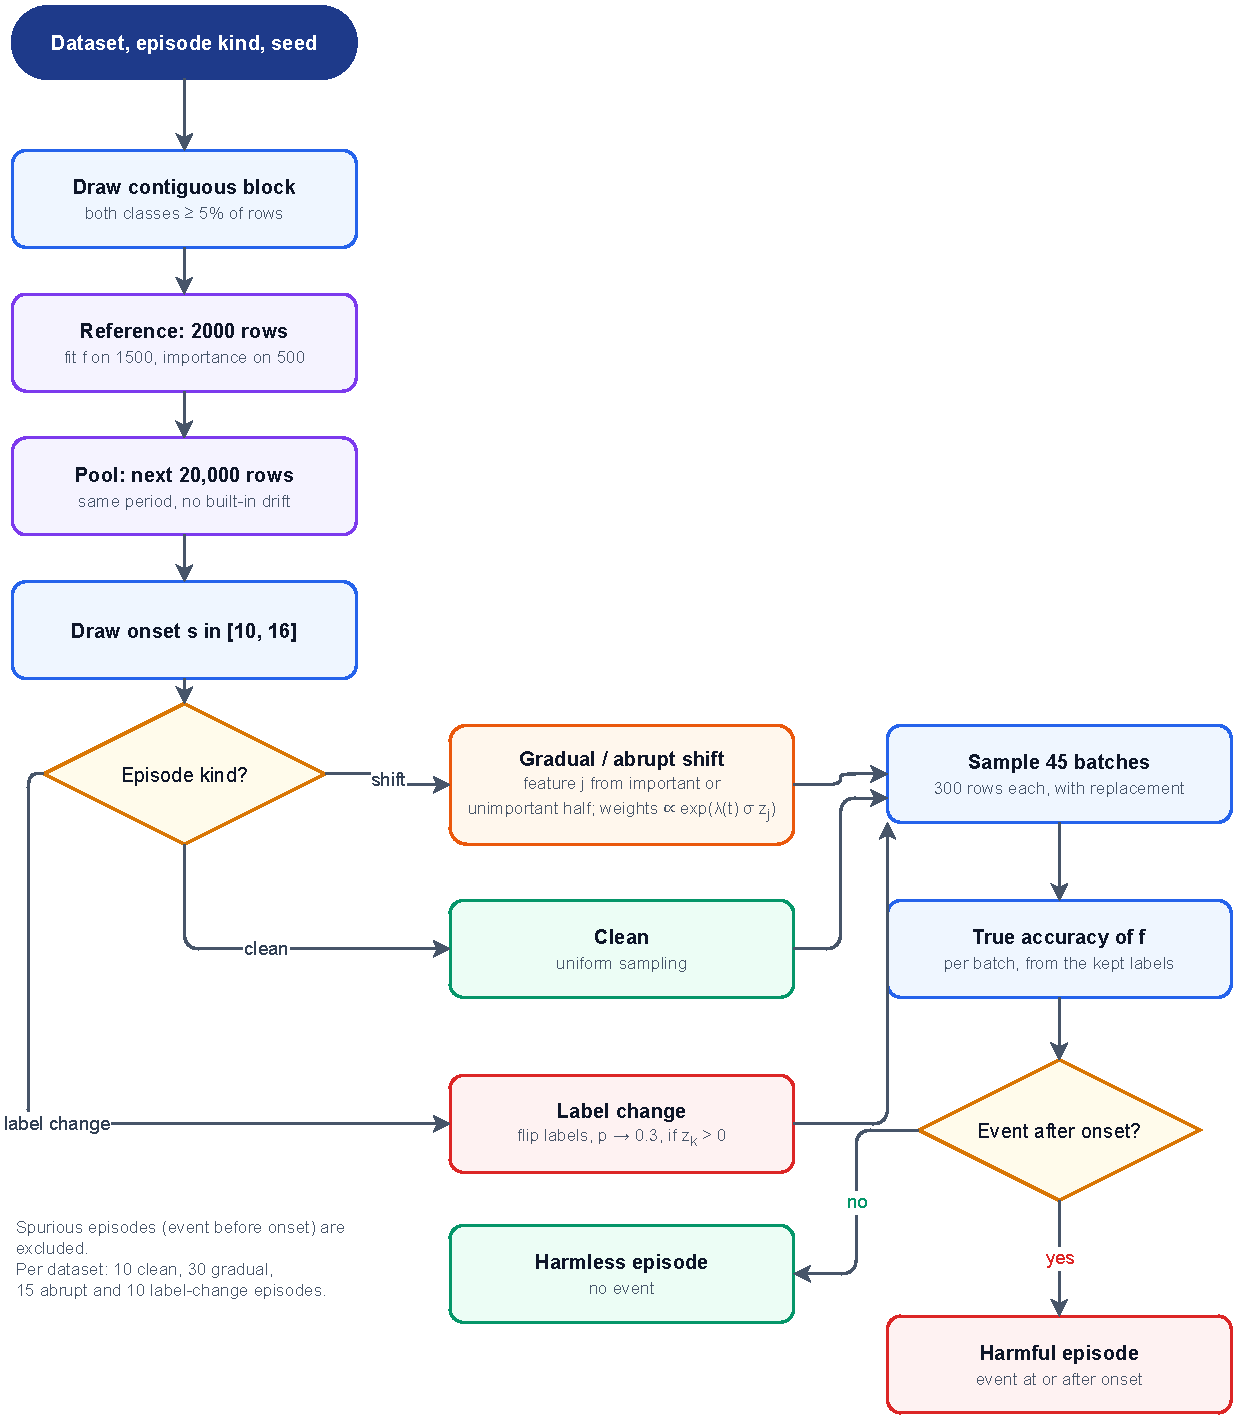
\includegraphics[width=0.82\textwidth]{fig_episode_generation.pdf}
\caption{Flowchart of benchmark episode generation.}
\label{fig:episode}
\end{figure}

\begin{algorithm}[H]
\caption{Building one benchmark episode}
\label{alg:episode}
\begin{algorithmic}[1]
\Require dataset $(X, y)$, episode kind, seed
\State draw a block start where both classes are $\geq$5\% of the fit rows and of the pool
\State $R \gets$ next 2000 rows; fit $f$ on the first 1500; permutation importance on the last 500
\State $P \gets$ next 20{,}000 rows (pool); draw onset $s \in [10,16]$
\If{kind is a shift} \State pick feature $j$ (important or unimportant half) and sign $\sigma$ \EndIf
\For{$t = 0, \dots, 44$}
  \If{kind is a shift and $t \geq s$}
    \State sample 300 rows of $P$ with weights $\propto \exp(\lambda(t)\,\sigma\, z_j)$
  \Else
    \State sample 300 rows of $P$ uniformly
  \EndIf
  \If{kind is a label change and $t \geq s$} \State flip labels of rows with $z_k > 0$ with probability $0.3\,\min(1, (t-s+1)/15)$ \EndIf
\EndFor
\State compute the accuracy of $f$ on every batch; label the episode harmful, harmless, clean or spurious
\end{algorithmic}
\end{algorithm}

\subsection{Datasets and data groups}
All datasets are binary (or reduced to majority class versus the rest) and use their first 20 non-constant features. \tabref{tab:groups} shows how they were used. The 13 v6 datasets had already been used as natural-order streams in the exploratory studies v1--v5; the confirmation groups of v7, v8 and v10 were downloaded only after the corresponding design was frozen and had never been used before. The full list is in Appendix~\ref{app:data}.

\begin{table}[H]
\caption{Data groups and their use (65 episodes per dataset).}
\label{tab:groups}
\centering
\small
\begin{tabular}{@{}lcl@{}}
\toprule
Group & Datasets & Use \\
\midrule
v6 development & 8 & design, thresholds and all later tuning \\
v6 held-out & 5 & one-time v6 verdict (seen in v1--v5 as natural streams) \\
v7 confirmation & 6 & one-time drift-watch verdict \\
v8 confirmation & 5 & one-time harm-tier verdict \\
v10 confirmation & 6 & one-time test of stricter alerting rules \\
Natural streams & 13 & 328 row-order windows, no injected shift (H5, C5) \\
\bottomrule
\end{tabular}
\end{table}

\section{Label-Free Signals}
\tabref{tab:signals_def} lists the signals computed for every batch without labels. They fall into two families. \emph{Input-shift} signals compare the batch's inputs with the reference; \emph{model-behaviour} signals describe how the model reacts to the batch.

\begin{table}[H]
\caption{Label-free signals computed per batch.}
\label{tab:signals_def}
\centering
\small
\begin{tabularx}{\textwidth}{@{}p{3.6cm}p{2.3cm}X@{}}
\toprule
Signal & Family & Definition \\
\midrule
Fused DEWS drift score & input shift & original prototype's weighted fusion of per-feature KS/PSI statistics, embedding MMD and a confidence component \\
Mean KS & input shift & mean two-sample KS statistic over features \\
Relevance-weighted shift & input shift & $\sum_j \text{importance}_j \cdot \mathrm{KS}_j$, using $f$'s permutation importance \\
Positive-rate shift & input shift & absolute change of the share of positive predictions from its burn-in mean \\
Confidence drop & behaviour & negative mean top-class probability of $f$ \\
Entropy & behaviour & mean prediction entropy of $f$ \\
Disagreement & behaviour & share of rows where $f$ disagrees with a random forest~\cite{breiman2001rf} and a gradient-boosting model~\cite{friedman2001gbm} trained on the same reference rows \\
\bottomrule
\end{tabularx}
\end{table}

\section{The Two-Tier Monitor}
\label{sec:twotier}
\figref{fig:twotier} shows how one batch flows through both tiers and how delayed labels later confirm or clear an alert.

\begin{figure}[H]
\centering
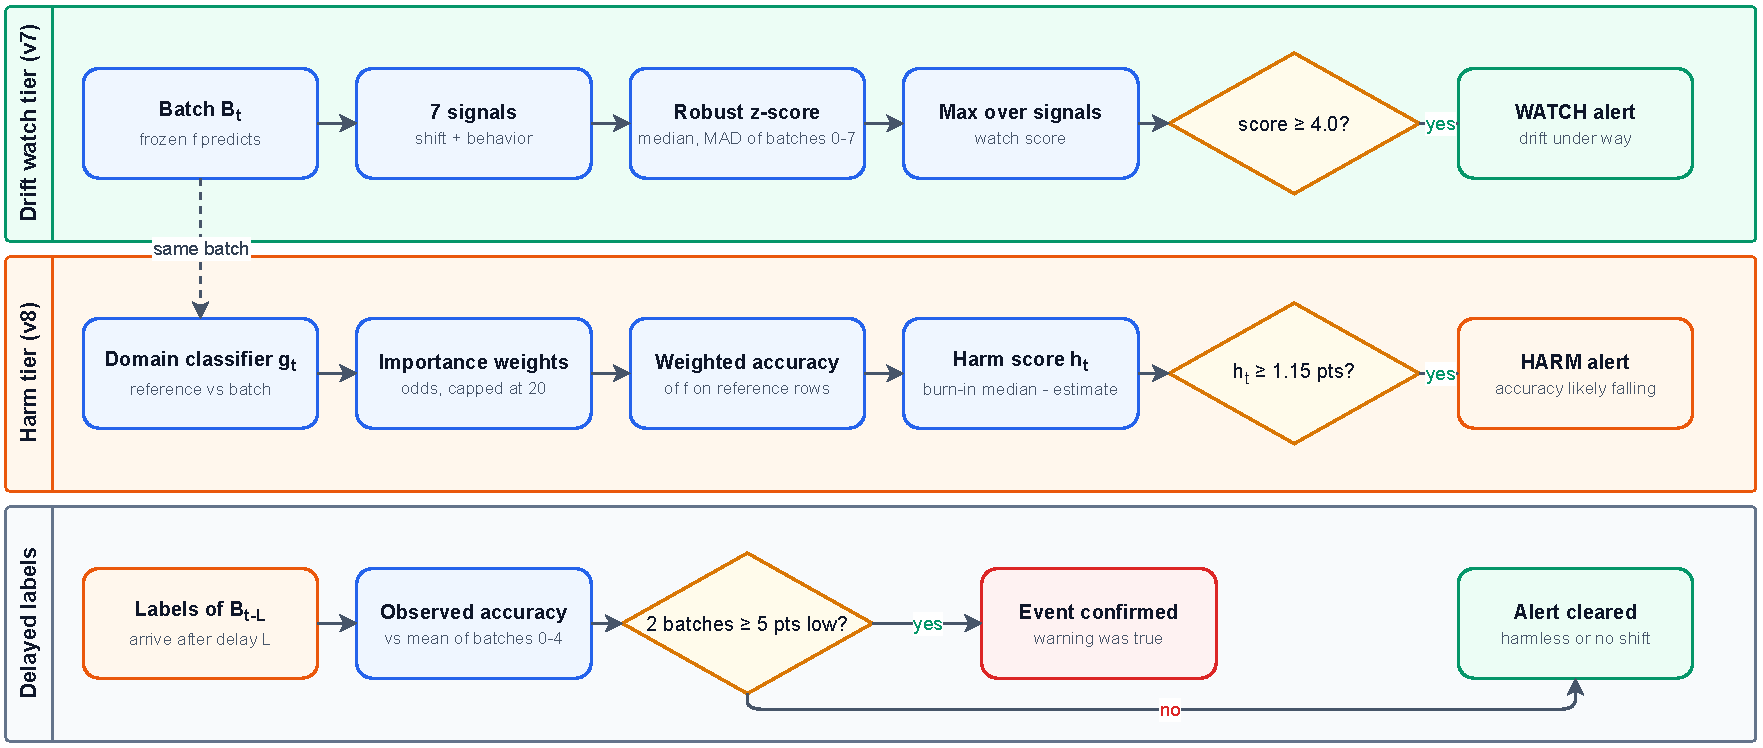
\includegraphics[width=\textwidth]{fig_two_tier_flow.pdf}
\caption{Per-batch data flow of the two-tier monitor and the confirmation by delayed labels.}
\label{fig:twotier}
\end{figure}

\subsection{Tier 1: drift watch (v7)}
Raw drift statistics live in dataset-specific units: a KS statistic of 0.1 may be normal noise on one dataset and a large shift on another. The drift watch therefore expresses every signal relative to the stream's own burn-in. For a signal $x_t$,
\begin{equation}
z_t = \frac{x_t - \mathrm{med}(x_{0:8})}{\max\left(1.4826\,\mathrm{MAD}(x_{0:8}),\ 0.01\right)},
\end{equation}
a robust z-score in which the median and the median absolute deviation (scaled to match a standard deviation for normal data) are computed on batches 0--7. The drift-watch score is the maximum $z_t$ over the seven signals of \tabref{tab:signals_def}. A WATCH alert is raised when the score exceeds \textbf{4.011} standard deviations, a threshold chosen on development data. Because the score is measured in deviations from the stream's own normal, the same threshold is comparable across streams that start in a stable period.

\subsection{Tier 2: harm tier (v8)}
\label{sec:harm}
Whether a shift harms the model depends on whether it moves the data into regions where this particular model is wrong. The labeled reference set shows where that is. For each batch $B_t$, a logistic domain classifier $g_t$ is trained to separate reference rows (label 0) from batch rows (label 1). For reference row $x_i$ with correctness $c_i = \mathbb{1}[f(x_i)=y_i]$, the importance weight and the label-free accuracy estimate are
\begin{equation}
w_i = \min\!\left(\frac{\rho_i}{\bar\rho},\ 20\right),\quad \rho_i=\frac{g_t(x_i)}{1-g_t(x_i)},\qquad \hat a_t = \frac{\sum_i w_i c_i}{\sum_i w_i},
\label{eq:iw}
\end{equation}
where $\bar\rho$ is the mean odds over the reference. Under covariate shift, $\hat a_t$ targets the accuracy of $f$ on $B_t$~\cite{shimodaira2000,sugiyama2007iwcv}. The harm score is the estimated drop since the burn-in,
\begin{equation}
h_t = \mathrm{med}(\hat a_{0:8}) - \hat a_t,
\end{equation}
in accuracy units. A HARM alert is raised when $h_t \ge 0.0115$ (an estimated drop of 1.15 accuracy points). The harm tier has no trained parameters beyond this threshold. Pure label changes are invisible to it by construction.

\subsection{Threshold selection}
Thresholds are chosen on development data only, with false alerts kept within 5 per 100 clean batches:
\begin{itemize}
\item \textbf{v6 rule} (also used by the drift watch): the threshold with the highest development T1 share; ties go to the higher threshold.
\item \textbf{Separation rule} (harm tier): the threshold that maximises the T2 share on harmful shifts minus the alert share on harmless shifts.
\end{itemize}

\section{Evaluation Protocol and Pre-Registration}
\label{sec:prereg}
Every experiment from v6 onward followed the workflow of \figref{fig:prereg}. Before any confirmation data were obtained, a configuration module defining the datasets, seeds, method, threshold rule and each hypothesis with its pass rule was committed to git. Thresholds were chosen on development data and frozen in JSON files whose SHA-256 fingerprints were recorded in the protocol; the confirmation script refuses to run if a fingerprint does not match. Deviations, for example shuffling a dataset whose rows are stored sorted by class, were logged with date and reason before any affected episode was built. Each verdict was then computed once, by a script that applies the frozen pass rules.

\begin{figure}[H]
\centering
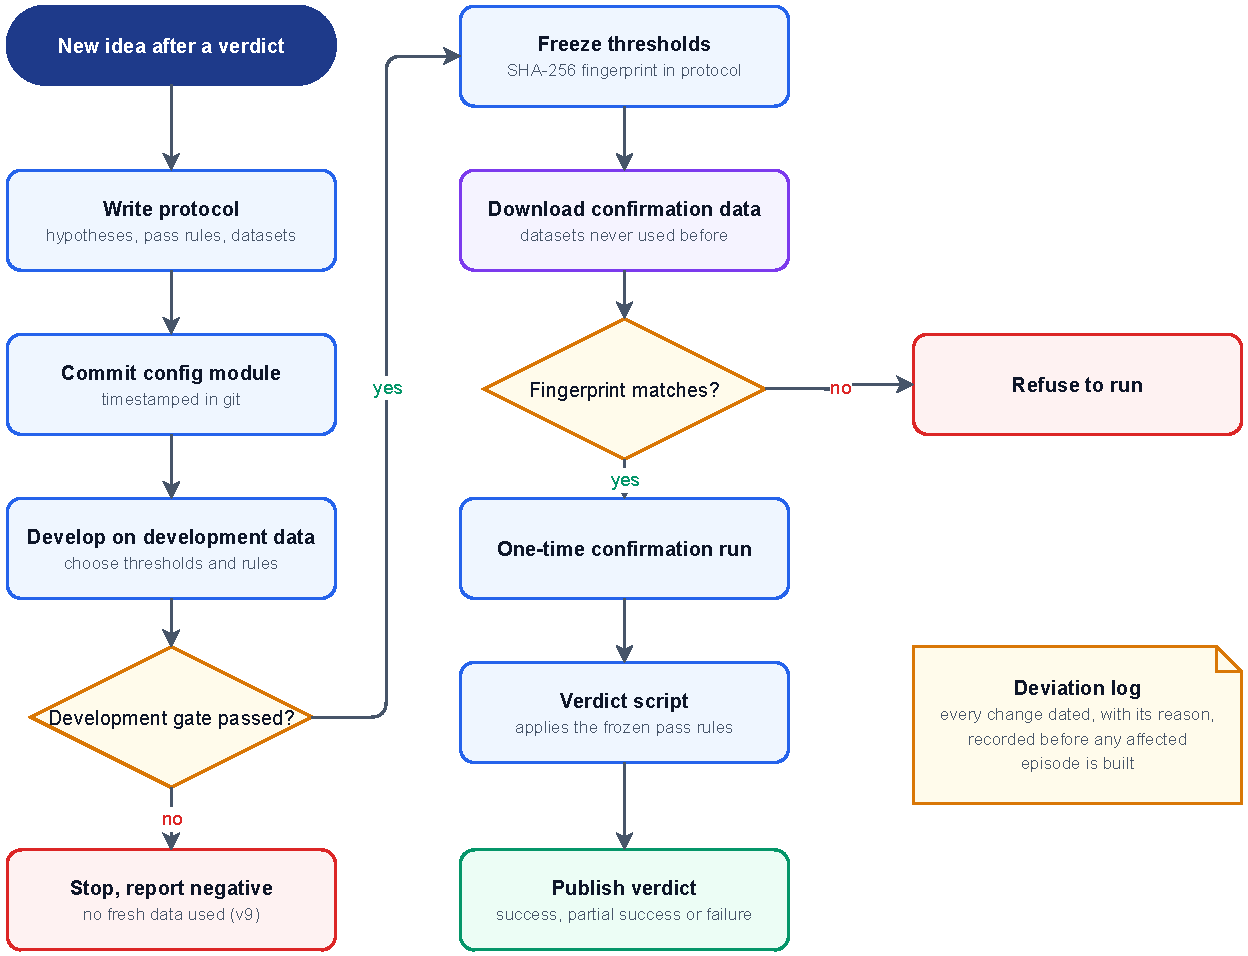
\includegraphics[width=0.92\textwidth]{fig_preregistration.pdf}
\caption{Pre-registration workflow used for every experiment from v6 onward.}
\label{fig:prereg}
\end{figure}

Confidence intervals are 95\% bootstrap intervals over episodes with 2000 resamples~\cite{efron1979bootstrap}; comparisons between two methods use a paired bootstrap that resamples the same episodes for both.

\section{Software Design}
\figref{fig:modules} shows the main parts of the code base and how they depend on each other. The core library \texttt{dews/} contains the benchmark, signal extraction, evaluation metrics, monitors and harm estimation. Experiment runners in \texttt{scripts/} use the library, read the frozen configurations and write all outputs to \texttt{artifacts/}. The dashboard, the paper figures and this report read only from \texttt{artifacts/}, so every number shown can be traced back to a saved result.

\begin{figure}[H]
\centering
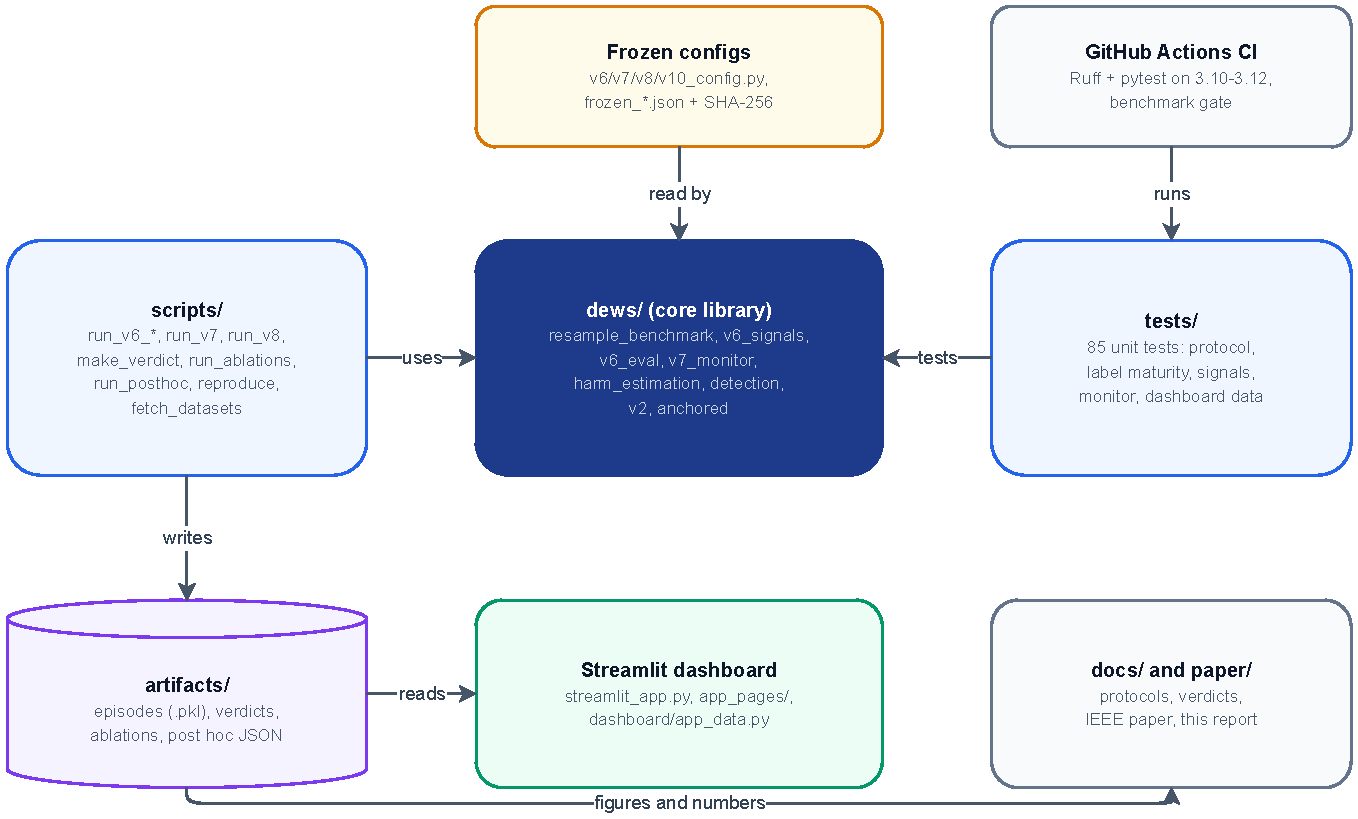
\includegraphics[width=0.9\textwidth]{fig_modules.pdf}
\caption{Software modules and their dependencies.}
\label{fig:modules}
\end{figure}

\subsection{Dashboard design}
The dashboard (\figref{fig:dashflow}) is a Streamlit~\cite{streamlit} application with four pages. A plain Python module, \texttt{dashboard/app\_data.py}, contains all data loading and replay logic without any Streamlit imports, so that it can be unit-tested. The \emph{replay} function reproduces exactly what the monitor knew at each batch: labels appear only after the selected delay, and scores are compared with the frozen thresholds.

\begin{figure}[H]
\centering
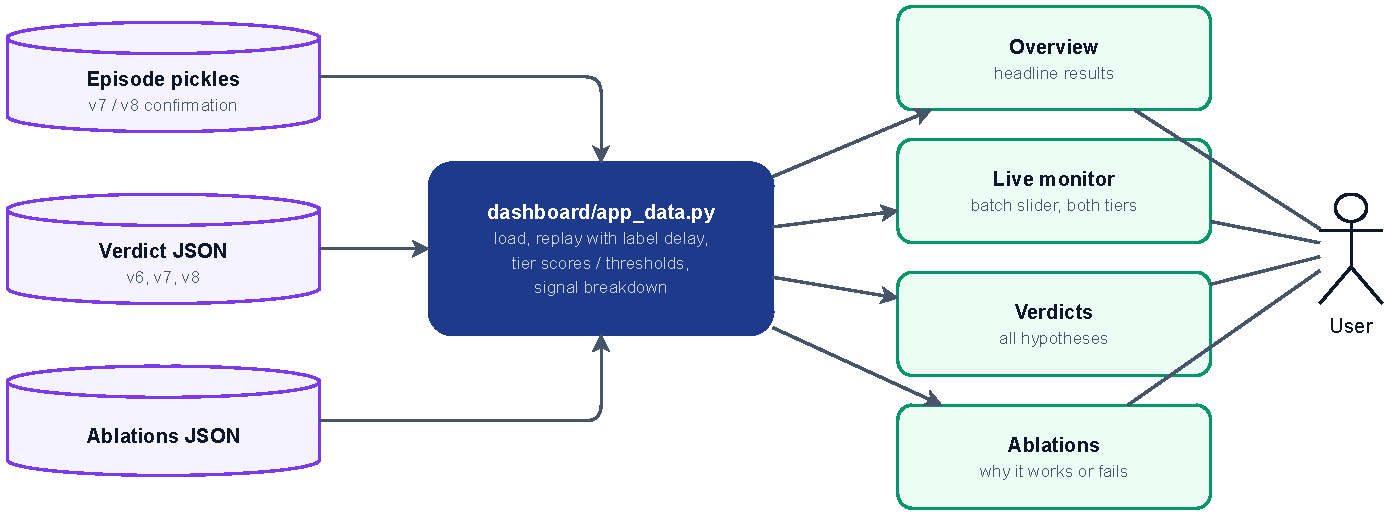
\includegraphics[width=0.95\textwidth]{fig_dashboard_flow.pdf}
\caption{Data flow of the Streamlit dashboard.}
\label{fig:dashflow}
\end{figure}
	% System design
%_____________________________________________________________________________________________
% Chapter 5: Implementation
%_____________________________________________________________________________________________

\chapter{Implementation}
\label{ch:impl}

\section{Tools and Technologies}
The system is written in Python. Models, auxiliary models and domain classifiers use scikit-learn~\cite{pedregosa2011sklearn}; statistics use NumPy and SciPy; tables use pandas; figures use matplotlib; and the dashboard uses Streamlit with Altair charts. Datasets are downloaded from OpenML~\cite{vanschoren2014openml}. The code is version-controlled with git and hosted on GitHub, where GitHub Actions runs linting, tests and a benchmark gate on every push. Diagrams were drawn with draw.io, and the paper and this report were typeset in \LaTeX.

\section{Development History: Ten Versions}
The final design was reached in ten versions (\figref{fig:evolution}). Versions v1--v5 were exploratory: they used synthetic scenarios and natural streams and were analysed after the fact. Versions v6--v10 were pre-registered (Section~\ref{sec:prereg}). Each version started from what had gone wrong in the previous one. Earlier results were kept as published.

\begin{figure}[H]
\centering
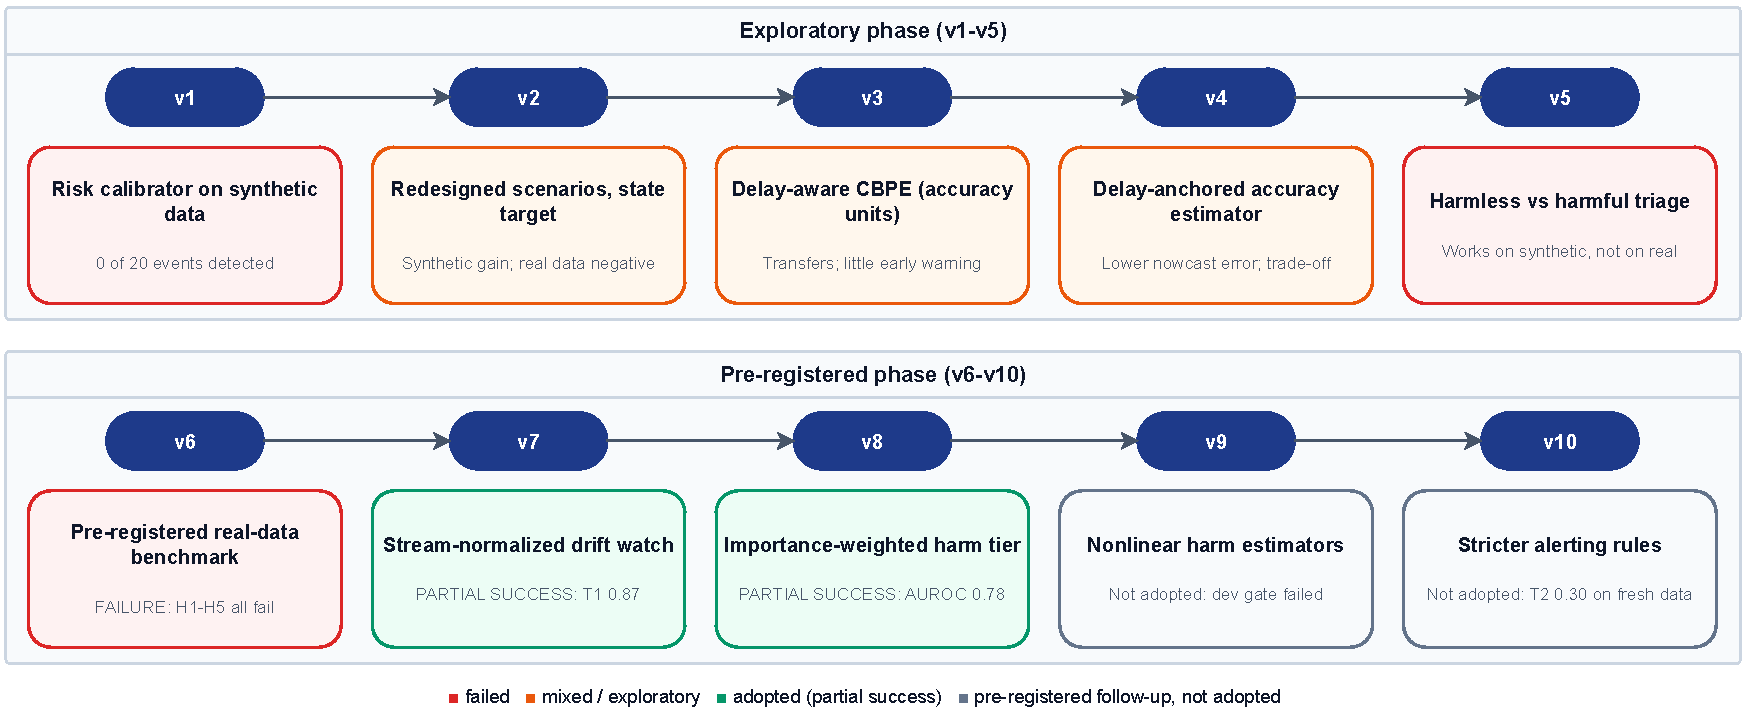
\includegraphics[width=\textwidth]{fig_evolution.pdf}
\caption{The ten versions of the system and what each showed.}
\label{fig:evolution}
\end{figure}

\subsection{v1: the original prototype's risk calibrator}
\label{sec:v1}
The first evaluation used controlled synthetic episodes (clean, harmless shift, gradual and abrupt harmful shift) with seeds split into training, validation and test groups, and label delays of 0, 2 and 5 batches. On 120 held-out episodes the learned risk calibrator matched \textbf{0 of 20} harmful events at every delay, while the fixed DEWS drift score matched 9 of 20, all after the event had started. We traced the failure to two design errors. In all 50 seeds the accuracy fell in the same batch as the intervention, so no monitor could have warned early. And the risk target (``an event \emph{starts} in the next 5 batches'') marked every batch after onset as negative, so the calibrator learned that more drift meant less risk.

\subsection{v2: redesigned scenarios and a state target}
\label{sec:v2}
v2 introduced noisy labels (baseline accuracy about 0.78), a randomised onset, relevant and nuisance features, a state target (``a degraded run starts or continues within the next 5 batches''), and a baseline that simply waits for delayed labels. On 250 held-out synthetic episodes the signals-only calibrator warned before onset in 98\% of harmful gradual episodes, about 4 batches ahead, where the fixed DEWS score gave no early warning (\tabref{tab:v2}). A leave-one-dataset-out study on four natural streams (electricity, airlines, covertype, bank-marketing), however, was negative: drift signals ranked accuracy risk weakly, and every signal-based threshold that met the budget on the other datasets raised 4--16 times more false alerts on the held-out one.

\begin{table}[H]
\caption{v2 controlled study, label delay $L=2$, 250 held-out synthetic episodes.}
\label{tab:v2}
\centering
\small
\begin{tabular}{@{}lcccc@{}}
\toprule
Method & Recall & Early-warning rate & AUROC & Brier \\
\midrule
Fixed DEWS score & 0.00 & 0.00 & 0.56 & -- \\
Confidence only & 0.44 & 0.27 & 0.50 & -- \\
Wait for delayed labels & 1.00 & 0.42 & 0.90 & -- \\
Calibrator, signals only & 0.73 & 0.42 & 0.83 & 0.161 \\
Calibrator, signals + matured accuracy & 1.00 & 0.56 & 0.94 & 0.086 \\
\bottomrule
\end{tabular}
\end{table}

\subsection{v3: delay-aware confidence-based estimation}
v3 expressed the score in accuracy units, which is what the event rule itself uses. It estimates each batch's accuracy as the mean top-class probability (as in CBPE) and corrects the bias with the residual of the latest 5 batches whose labels have already arrived. On four unseen natural streams this delay-aware CBPE stayed at 0.3--7 false alerts per 100 clean batches, against 10--11 for the drift scores, a first sign that units matter. It did not, however, give more early warning than waiting for labels.

\subsection{v4: delay-anchored accuracy estimation}
v4 anchored the estimate on the last matured accuracy and corrected it with a ridge regression on the change in 11 label-free signals, including disagreement with auxiliary models trained on the same reference rows. Disagreement turned out to be the most informative label-free error signal (mean within-window Spearman correlation 0.41 with error, against 0.19 for confidence drop). The estimator reduced nowcast error compared with stale labels, increasingly with delay (\figref{fig:nowcast}), but against waiting for labels it was a trade-off rather than a win.

\begin{figure}[H]
\centering
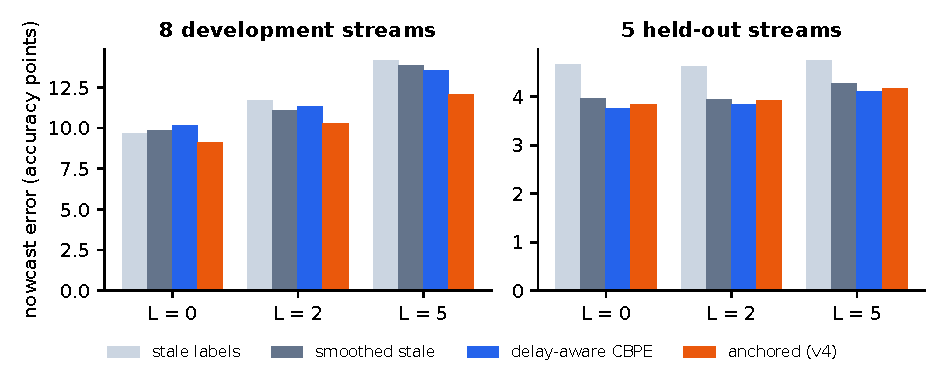
\includegraphics[width=\textwidth]{ch_v4_nowcast.pdf}
\caption{v4 accuracy nowcast error (mean absolute error in accuracy points) on 8 development streams (leave-one-dataset-out) and 5 held-out streams, by label delay.}
\label{fig:nowcast}
\end{figure}

\subsection{v5: harmless versus harmful shifts}
v5 asked whether the monitor could tell harmful from harmless shifts. A relevance-weighted shift, $\sum_j \text{importance}_j\cdot\mathrm{KS}_j$, separated them perfectly on synthetic data (AUROC 1.0), where harmlessness meant ``this feature does not matter''. On 13 real streams it did not (AUROC 0.53 on held-out streams). A sustained-alert rule did not help either. This is why v6 moved to real data with a pre-registered protocol.

\subsection{v6--v10: pre-registered experiments}
v6 built the re-sampling benchmark of Section~\ref{sec:benchmark} and evaluated a delay-aware risk calibrator under a full pre-registered protocol. It failed, and its diagnosis (thresholds in raw units do not transfer) led to the stream-normalised drift watch of v7. v7's second tier failed to separate harm, which led to the reference-based harm tier of v8. v9 and v10 tried to improve the harm tier and were not adopted. The results are reported in Chapter~\ref{ch:results}.

\section{Code Structure}
\tabref{tab:code} lists the main modules of the final system.

\begin{table}[H]
\caption{Main modules of the code base.}
\label{tab:code}
\centering
\small
\begin{tabularx}{\textwidth}{@{}p{5.3cm}X@{}}
\toprule
Module & Responsibility \\
\midrule
\texttt{dews/resample\_benchmark.py} & builds benchmark episodes from real datasets (Algorithm~\ref{alg:episode}) \\
\texttt{dews/v6\_signals.py} & per-batch signal extraction with each episode's monitored model and auxiliary models \\
\texttt{dews/v6\_eval.py} & event rule, warning tiers, false alerts, AUROC, threshold selection, v6 calibrator \\
\texttt{dews/v7\_monitor.py} & robust normalisation and the drift-watch score \\
\texttt{dews/harm\_estimation.py} & importance-weighted reference accuracy and the harm score \\
\texttt{dews/v6/v7/v8\_config.py} & frozen protocols: datasets, seeds, hypotheses, pass rules \\
\texttt{dews/detection.py}, \texttt{monitoring.py} & original DEWS detectors (KS, PSI, JSD, MMD, confidence) and fused score \\
\texttt{dews/v2.py}, \texttt{anchored.py} & exploratory library (v2--v4), delay-anchored estimator \\
\texttt{scripts/run\_v6\_*.py}, \texttt{run\_v7.py}, \texttt{run\_v8.py} & development, freezing, download, extraction and one-time confirmation \\
\texttt{scripts/make\_verdict.py} & applies the v6 pass rules and writes the verdict \\
\texttt{scripts/run\_ablations.py}, \texttt{run\_posthoc.py} & ablations and post hoc baselines \\
\texttt{scripts/reproduce.py} & one-command rebuild and verification of all verdicts \\
\texttt{streamlit\_app.py}, \texttt{app\_pages/}, \texttt{dashboard/} & the dashboard \\
\texttt{tests/} & unit tests \\
\bottomrule
\end{tabularx}
\end{table}

\section{Key Implementation Details}
\subsection{Enforcing label delay}
All label-derived features are computed from a helper that receives the current batch index and the delay and returns only the accuracies of batches $b \le t-\max(L,1)$. The same rule is used by the replay in the dashboard. Unit tests change the labels of batches that have not yet matured and check that no score at time $t$ changes.

\subsection{Per-batch monitoring}
Algorithm~\ref{alg:monitor} shows the per-batch logic of the final two-tier monitor.

\begin{algorithm}[H]
\caption{Two-tier monitoring of one stream}
\label{alg:monitor}
\begin{algorithmic}[1]
\Require frozen $f$, reference $(X_R, y_R)$, thresholds $\tau_W=4.011$, $\tau_H=0.0115$, delay $L$
\State $c_i \gets \mathbb{1}[f(x_i)=y_i]$ for every reference row
\For{each batch $B_t$}
  \State compute the 7 signals $x_t^{(k)}$ from $B_t$, $f$ and the auxiliary models
  \State fit domain classifier $g_t$ on $X_R$ (label 0) versus $B_t$ (label 1)
  \State $w_i \gets \min(\rho_i/\bar\rho, 20)$; \quad $\hat a_t \gets \sum_i w_i c_i / \sum_i w_i$
  \If{$t \geq 8$}
    \State $z^{(k)}_t \gets (x^{(k)}_t - \mathrm{med}(x^{(k)}_{0:8})) / \max(1.4826\,\mathrm{MAD}(x^{(k)}_{0:8}), 0.01)$
    \State \textbf{if} $\max_k z^{(k)}_t \geq \tau_W$ \textbf{then} raise WATCH
    \State \textbf{if} $\mathrm{med}(\hat a_{0:8}) - \hat a_t \geq \tau_H$ \textbf{then} raise HARM
  \EndIf
  \State release labels of $B_{t-\max(L,1)}$; update observed accuracy; confirm or clear alerts by the event rule
\EndFor
\end{algorithmic}
\end{algorithm}

\subsection{Pre-registration in code}
Each pre-registered experiment has its own configuration module in \texttt{dews/} (for example \texttt{v7\_config.py}; the v10 module is on its branch) that defines the datasets, seeds, settings and every hypothesis with its pass rule; a unit test checks the v6 configuration. Development scripts write the chosen thresholds to \texttt{artifacts/vN/frozen\_vN.json}. The first 16 hexadecimal digits of the file's SHA-256 hash are recorded in the protocol document, and the confirmation script computes the hash again and refuses to run if it is not found there. Downloads of confirmation datasets are separate commands that were run only after this commit.

\subsection{Parallel extraction}
Signal extraction trains several models per batch and dominates the run time. Extraction runs as six independent shard processes, each writing its own result file, which are merged before evaluation. Rebuilding everything from scratch takes about two hours on the development laptop.

\section{Dashboard}
The dashboard has four pages. The \emph{Overview} (\figref{fig:scr_overview}) summarises the main results. The \emph{Live monitor} (\figref{fig:scr_live}) replays a saved episode batch by batch: the user chooses the data group, dataset, episode type and label delay, and moves a slider over the batches. Key moments are shown as metrics (shift start, accuracy event, first drift-watch alert, first harm warning, label confirmation), with both tier scores divided by their thresholds, the accuracy seen through delayed labels, the label-free harm estimate, and a breakdown of which signals moved. The \emph{Verdicts} page lists every pre-registered hypothesis with its result, and \emph{Why it works} presents the ablation findings.

\begin{figure}[H]
\centering
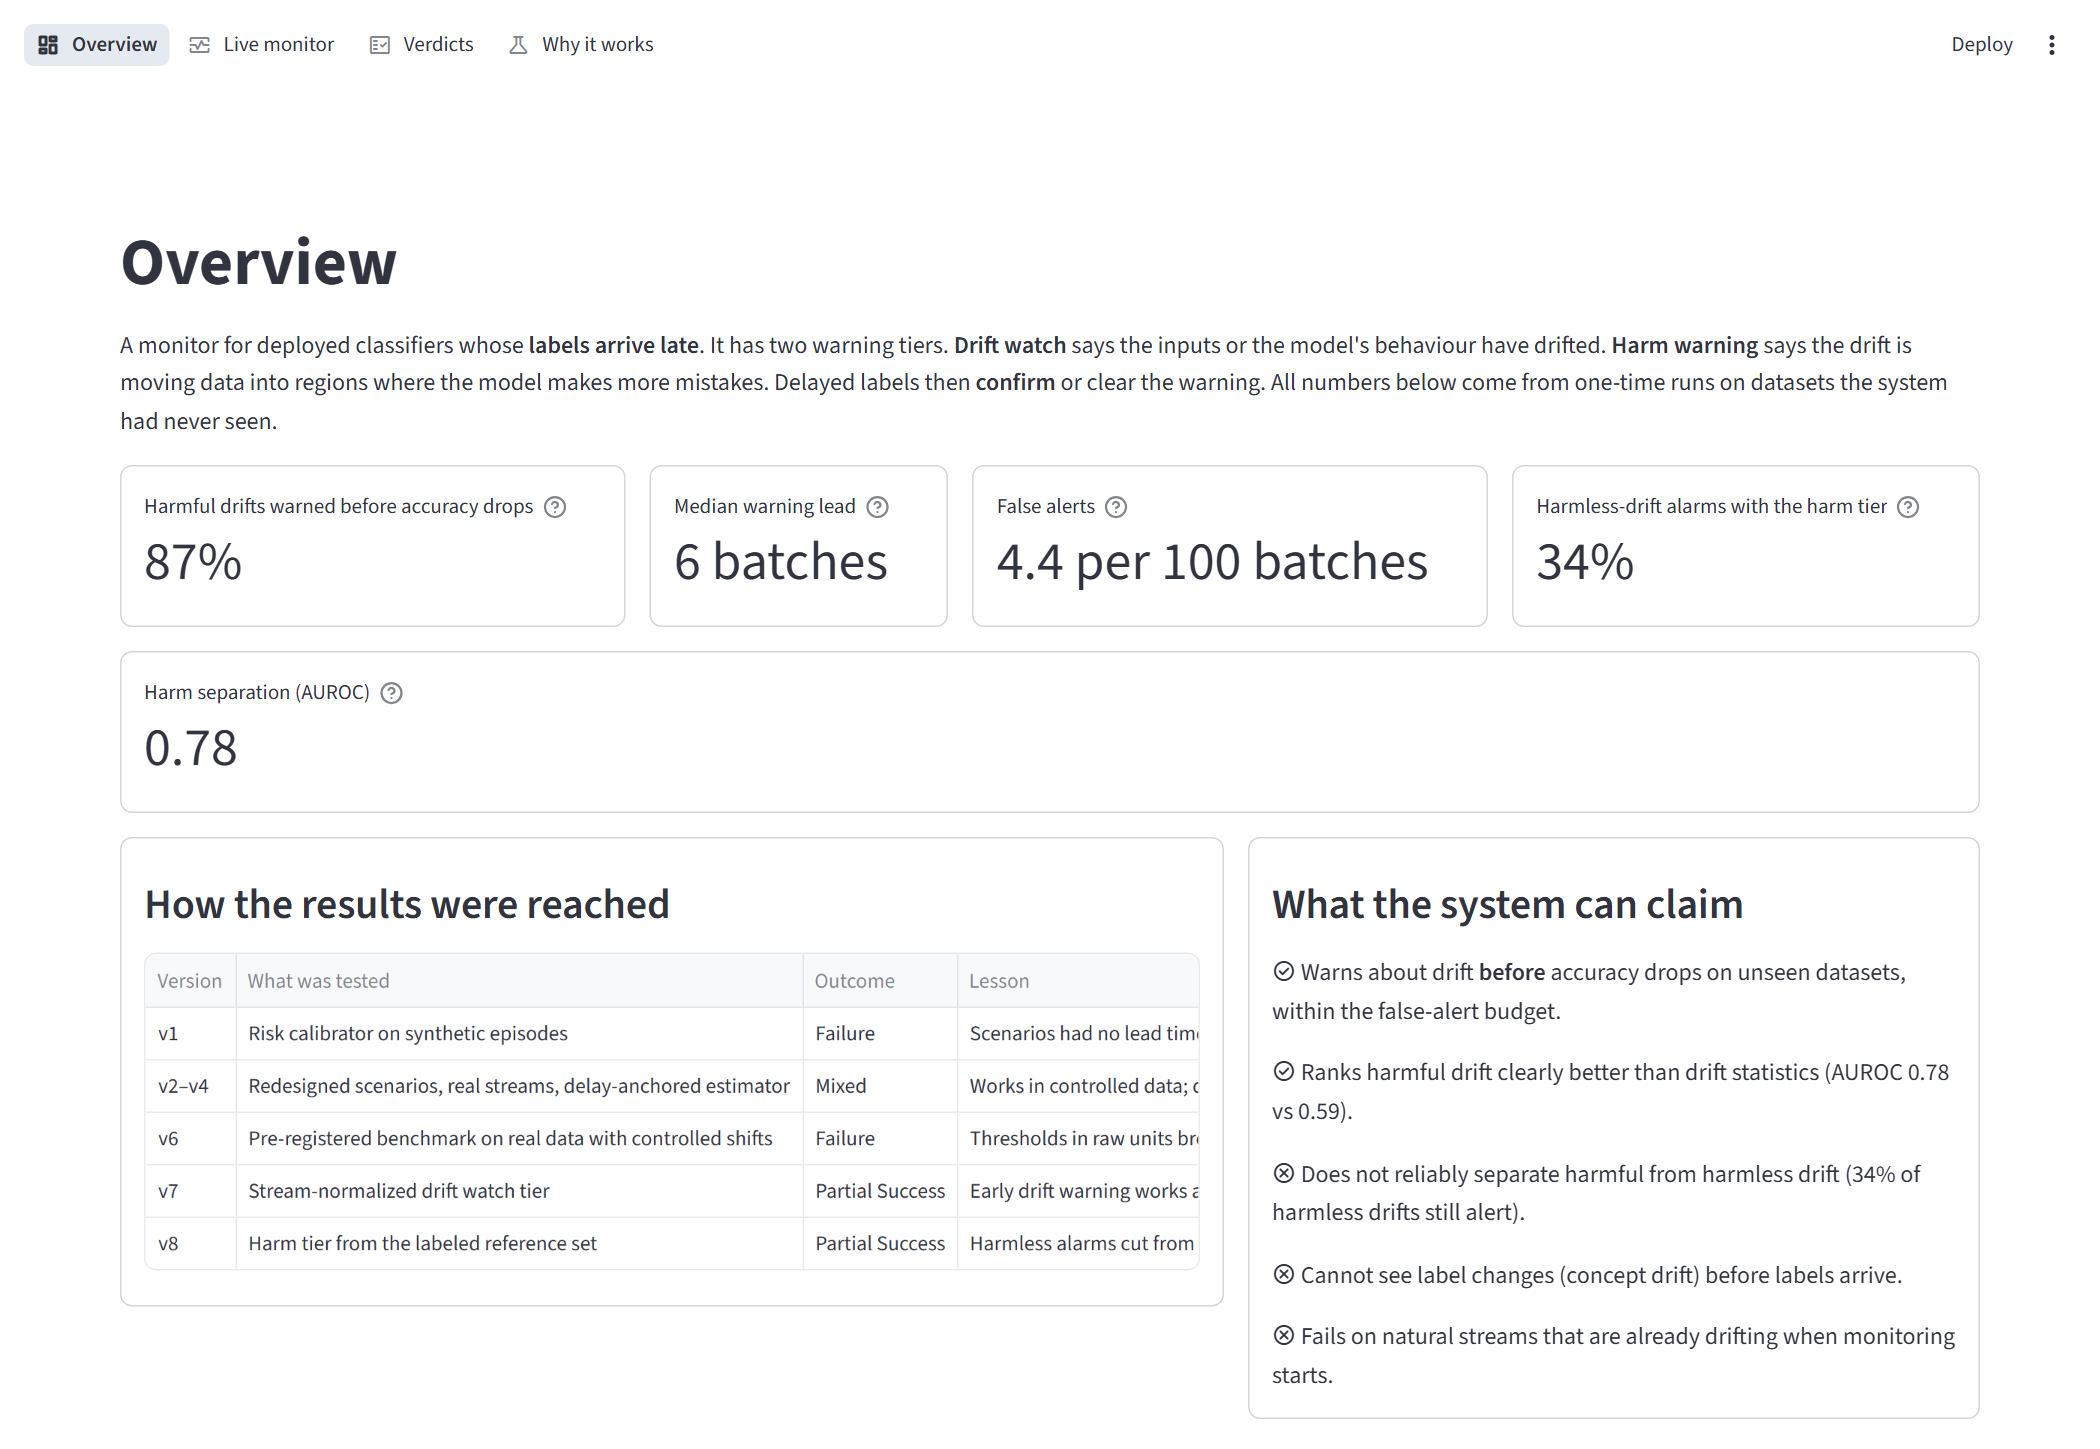
\includegraphics[width=0.92\textwidth]{overview.png}
\caption{Dashboard: Overview page.}
\label{fig:scr_overview}
\end{figure}

\begin{figure}[H]
\centering
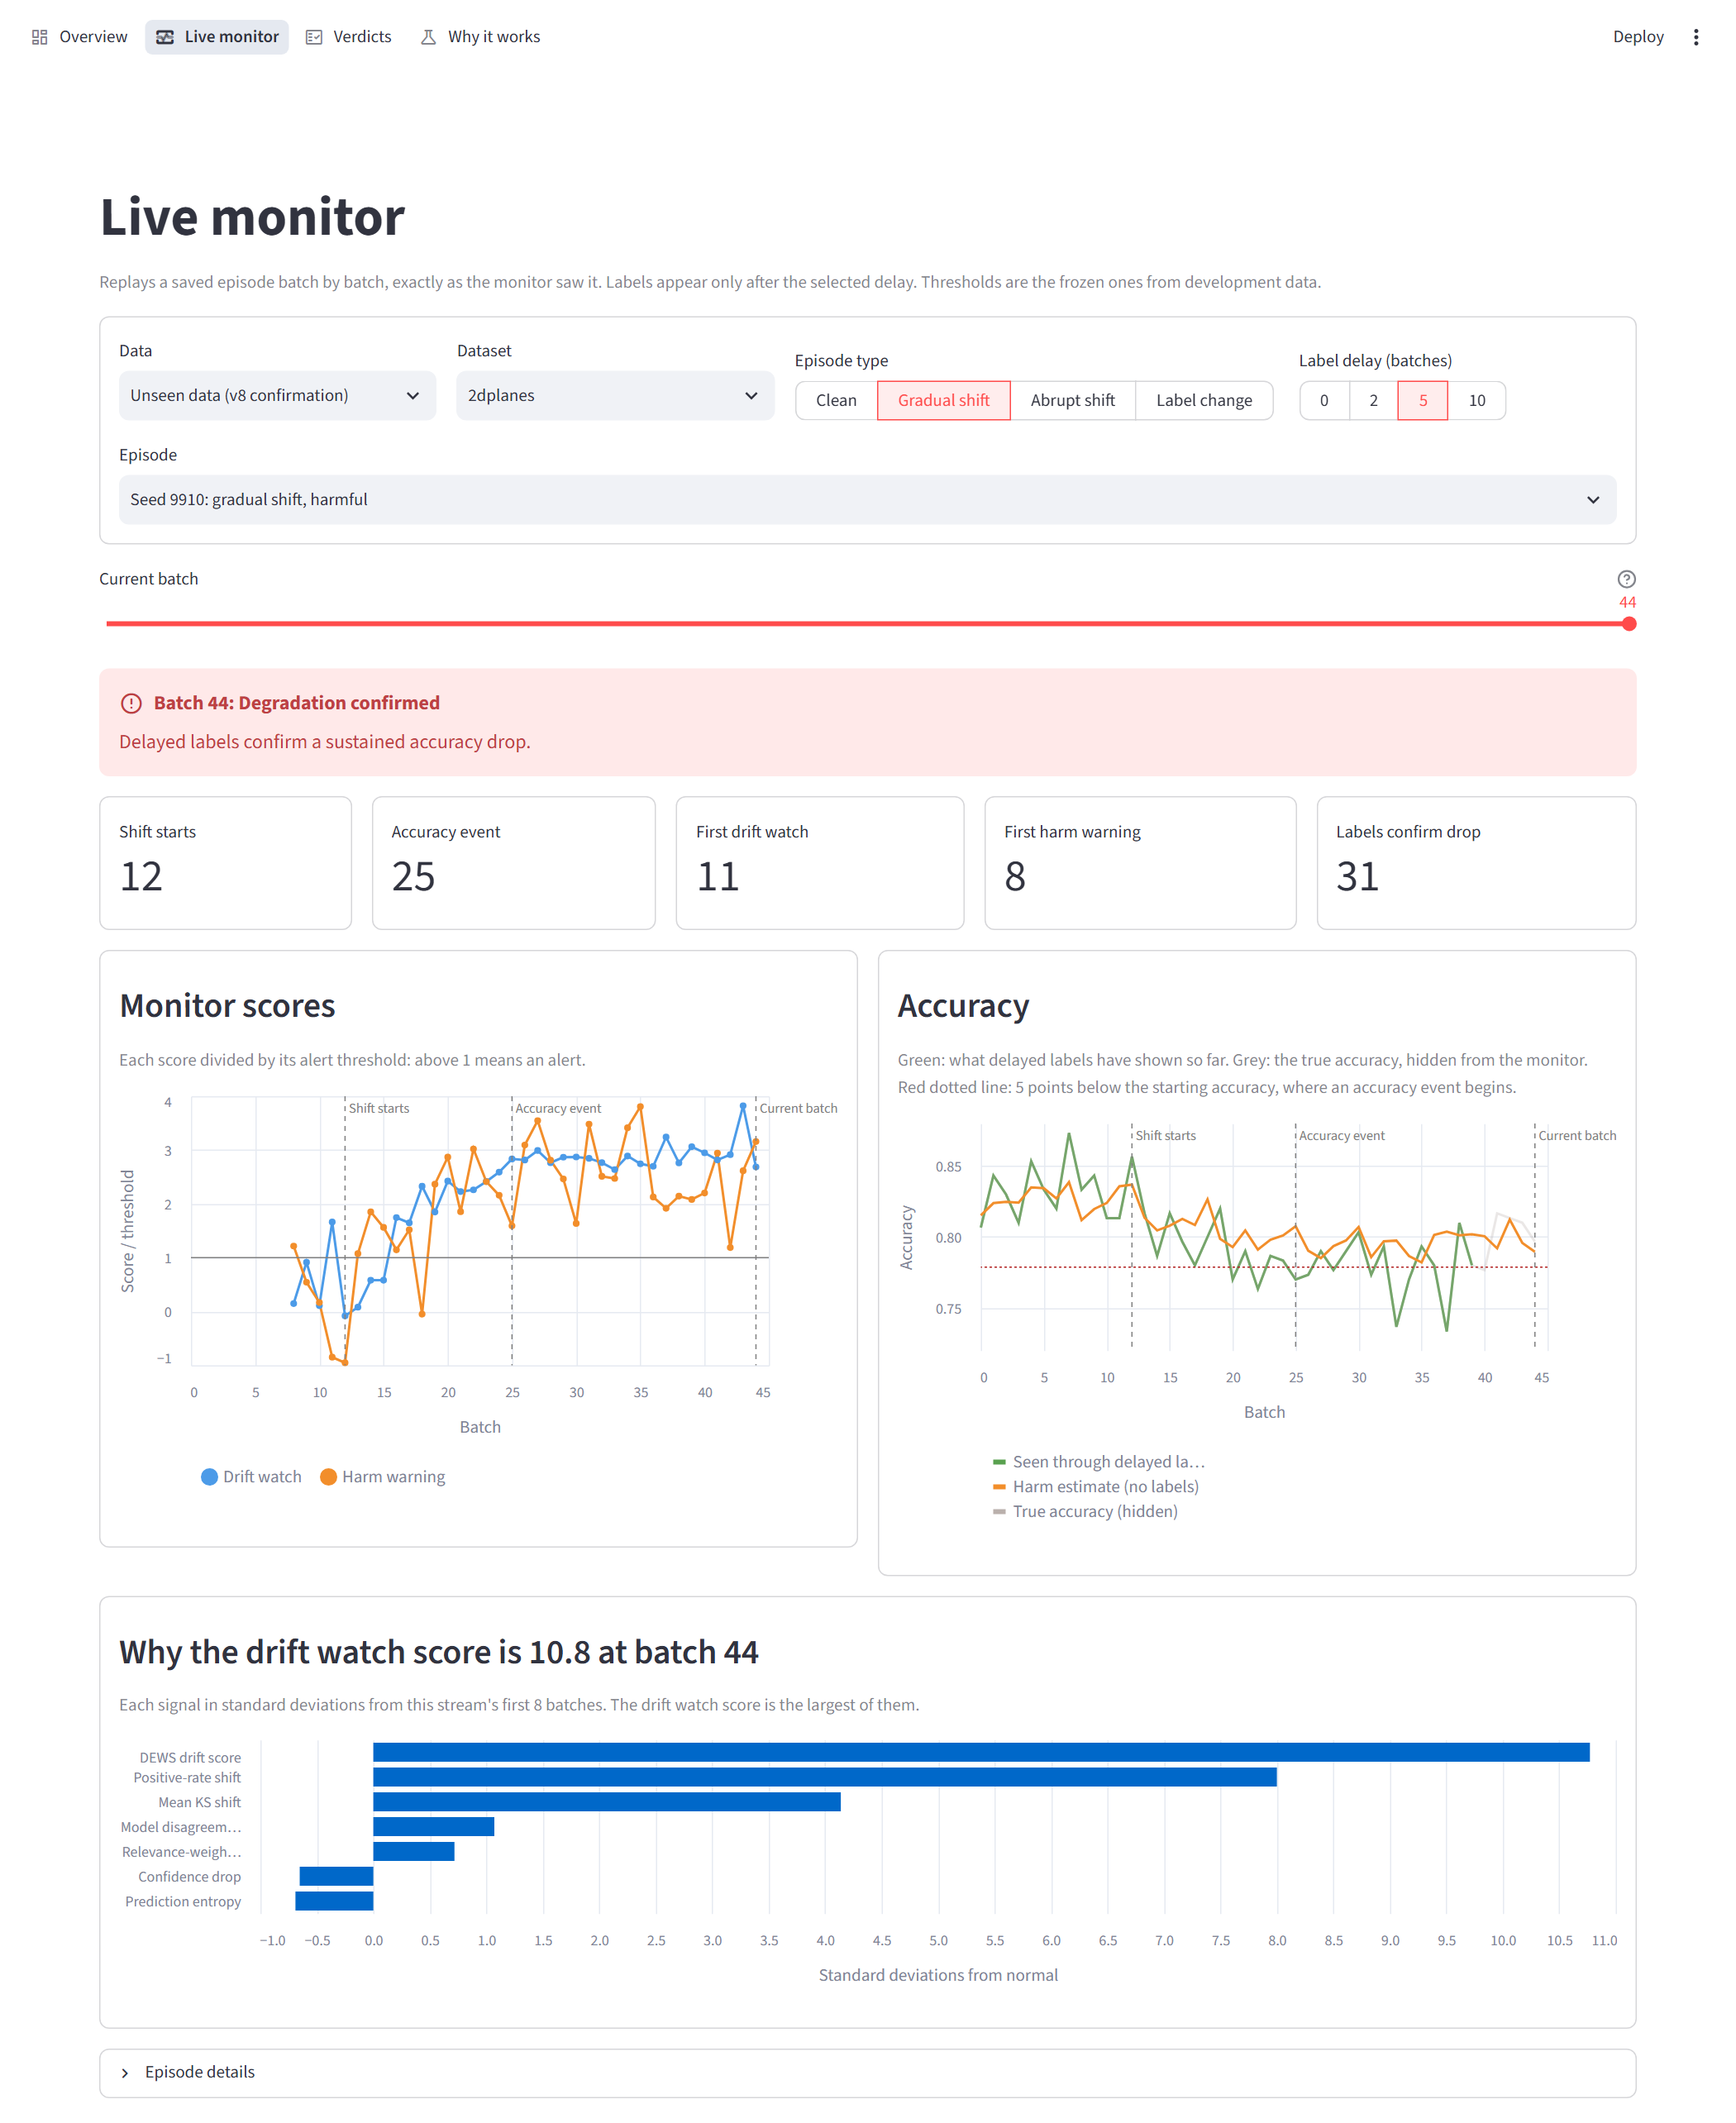
\includegraphics[width=0.8\textwidth]{live_monitor.png}
\caption{Dashboard: Live monitor replaying a harmful gradual shift on an unseen dataset (2dplanes, label delay 5). Alerts before the shift at batch 12 count as false alerts in the evaluation.}
\label{fig:scr_live}
\end{figure}

\begin{figure}[H]
\centering
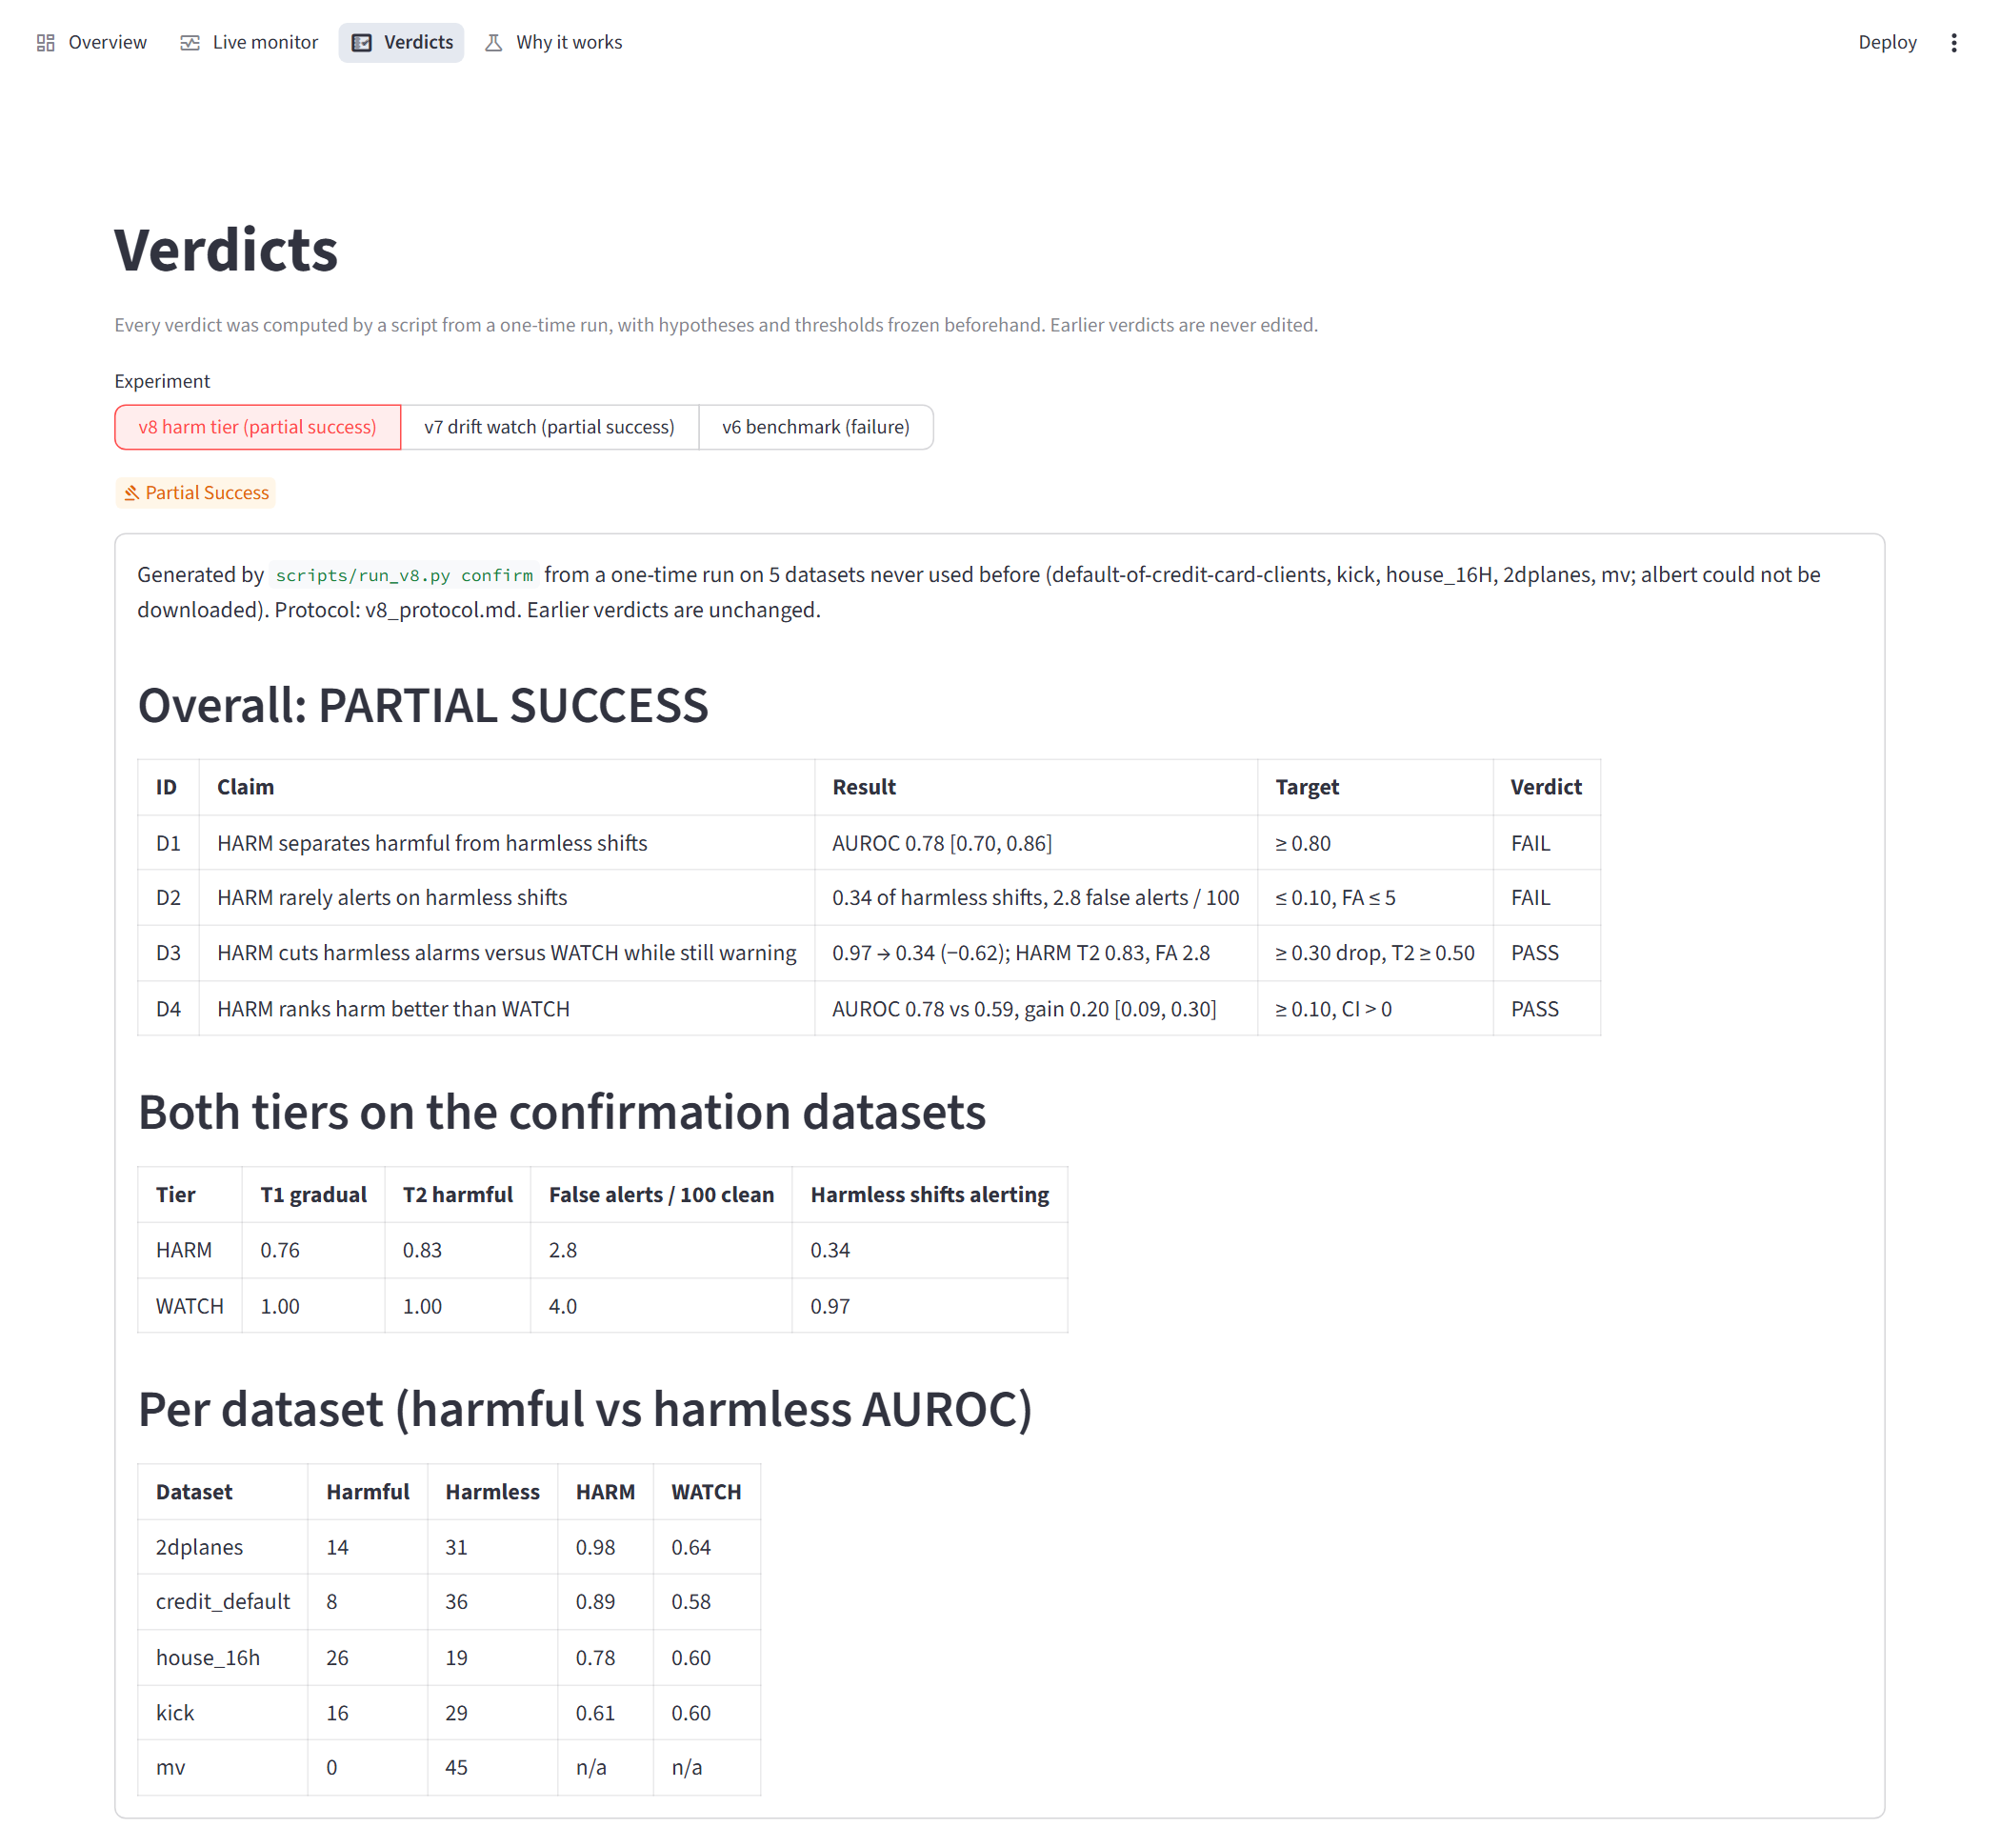
\includegraphics[width=0.85\textwidth]{verdicts.png}
\caption{Dashboard: Verdicts page.}
\label{fig:scr_verdicts}
\end{figure}

\begin{figure}[H]
\centering
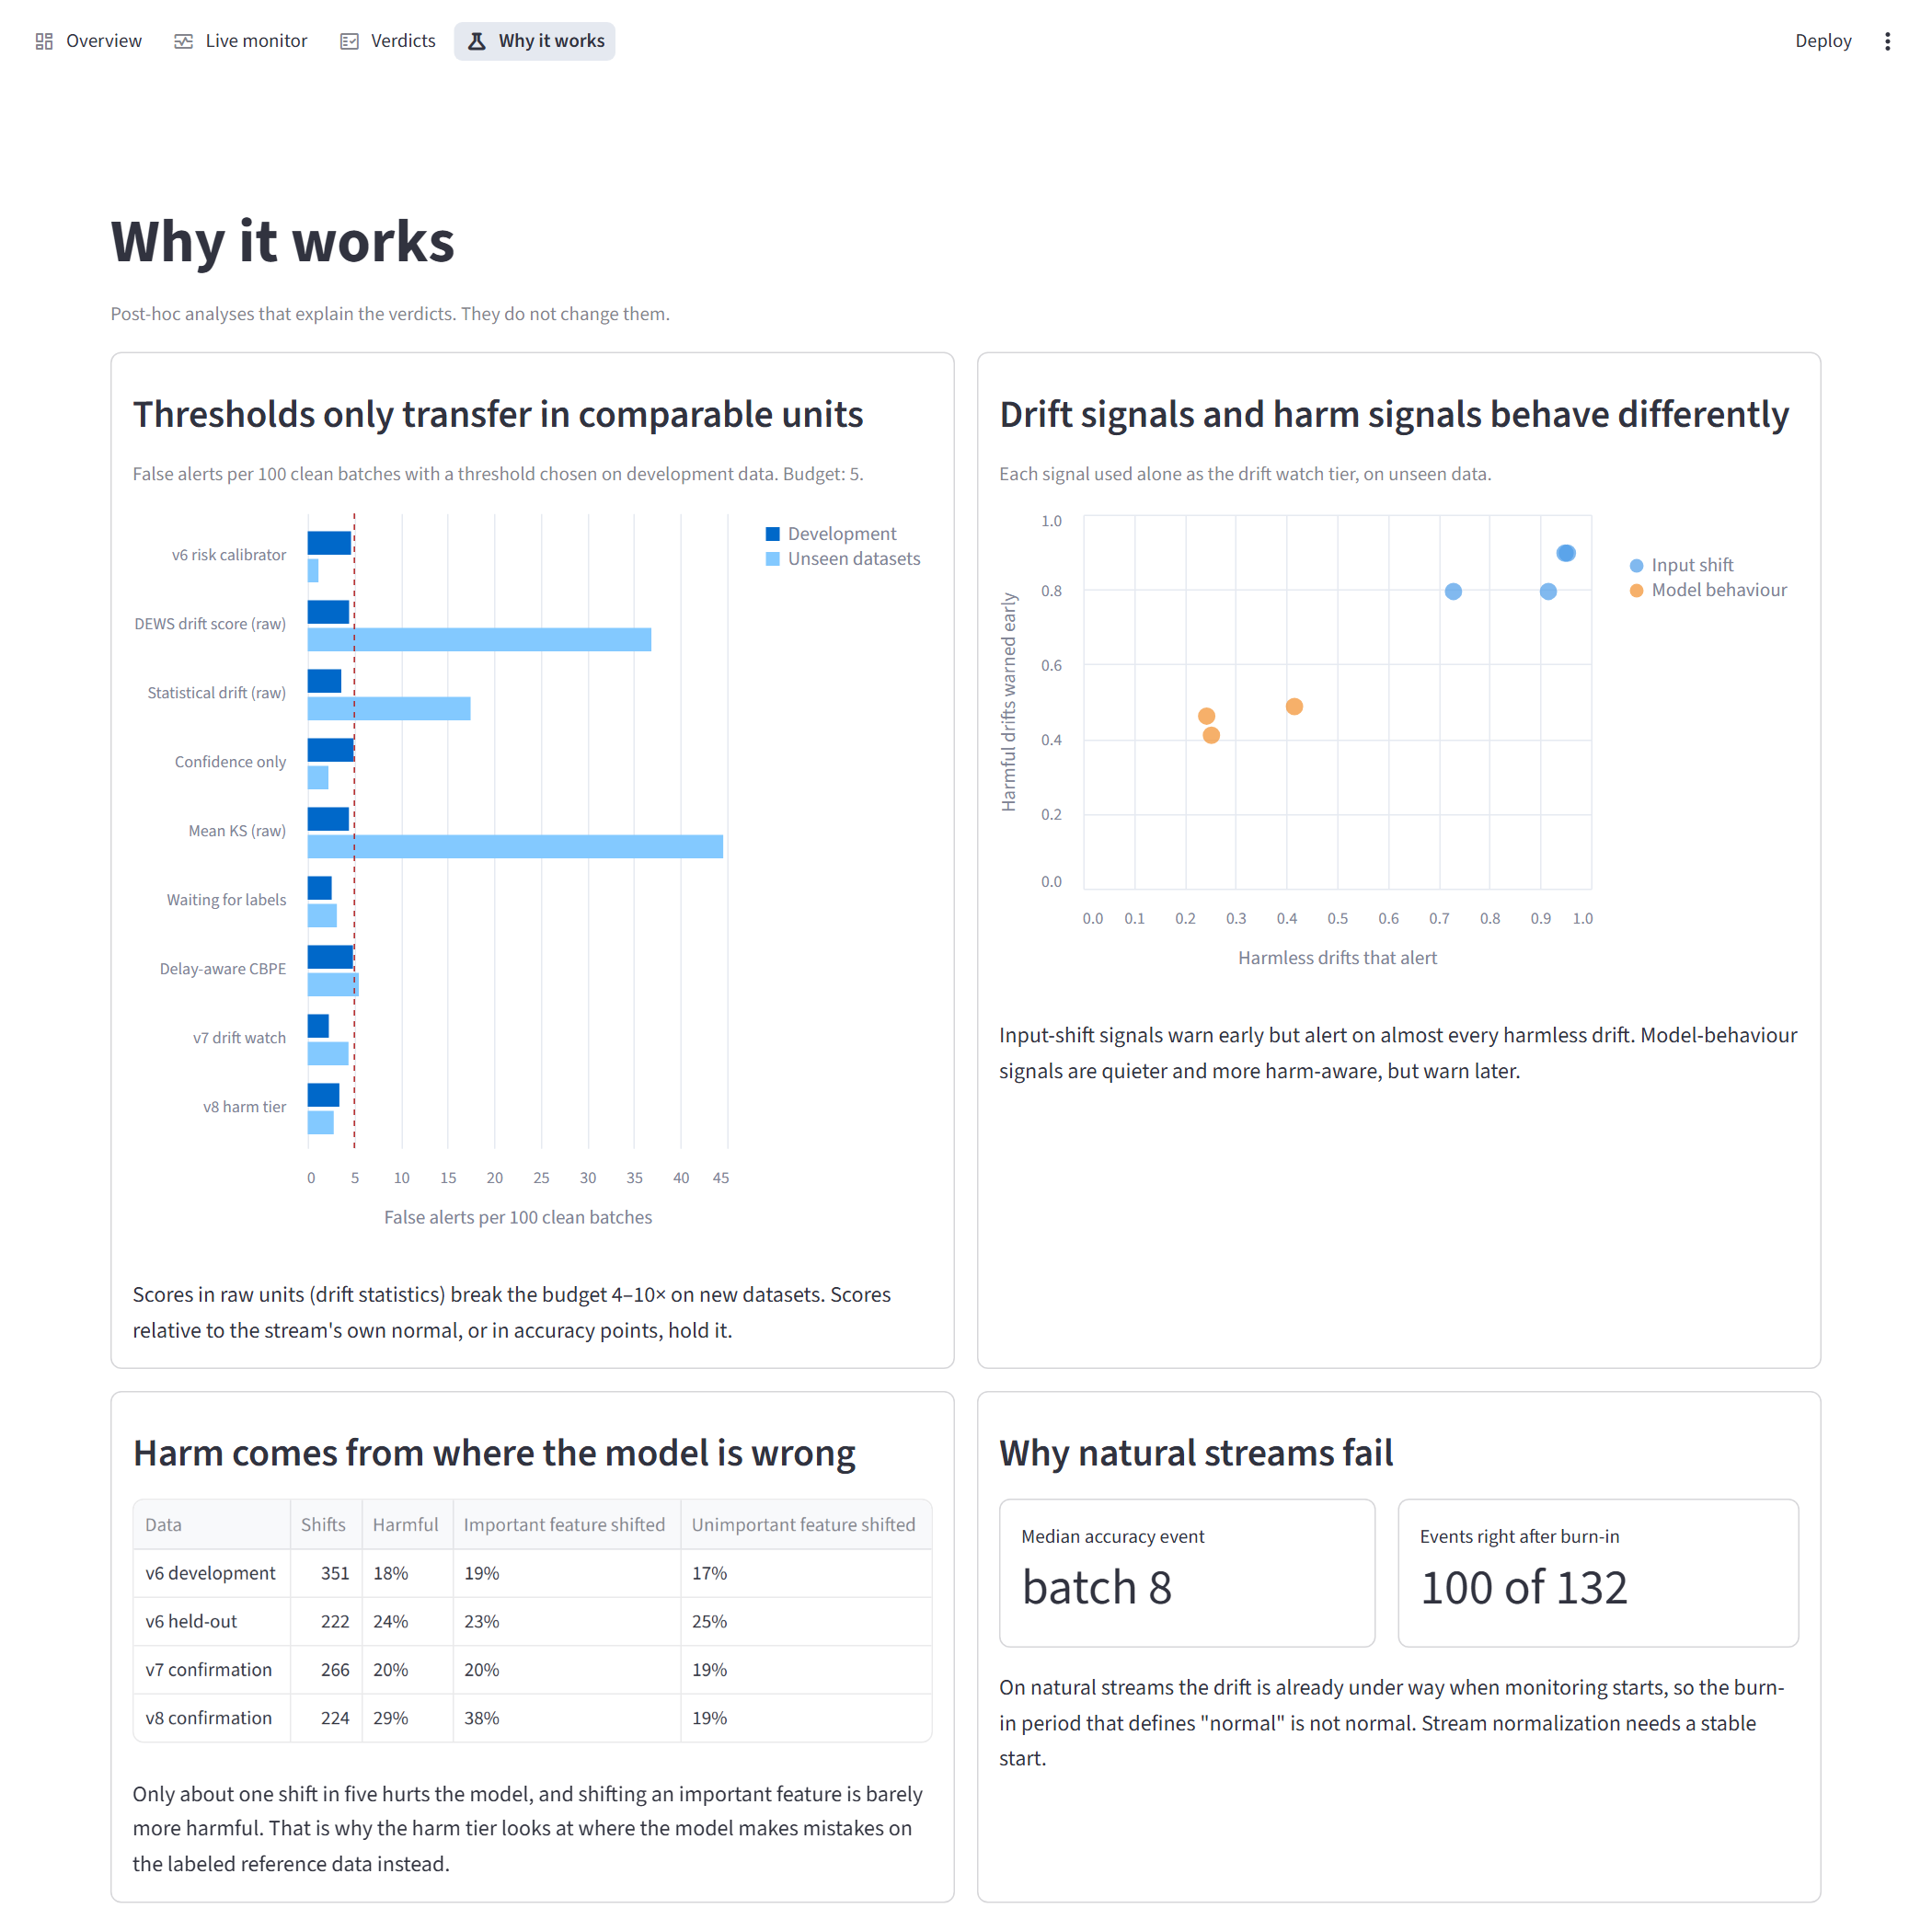
\includegraphics[width=0.85\textwidth]{ablations.png}
\caption{Dashboard: ``Why it works'' page with the ablation findings.}
\label{fig:scr_ablations}
\end{figure}

\section{Testing and Continuous Integration}
\label{sec:tests}
The repository contains 85 unit tests. They cover the protocol configuration, the event rule and warning tiers, label maturity (no score may change when unmatured labels change), the benchmark generator, signal extraction, the v7 monitor, the dashboard's data and replay logic, and components of the original prototype (detectors, alerts, forecasting, storage). The API tests of the legacy FastAPI service are skipped when that optional component is not installed.

GitHub Actions runs on every push and pull request (\figref{fig:ci}): it installs the core requirements, runs Ruff (pinned to version 0.17.4) and the full test suite on Python 3.10, 3.11 and 3.12, and then runs a benchmark gate that checks the legacy detector's lag, alert count and accuracy. In the CI run for the final code (10 November 2026) all jobs passed, with 84 tests passed and 1 skipped on each Python version.

\begin{figure}[H]
\centering
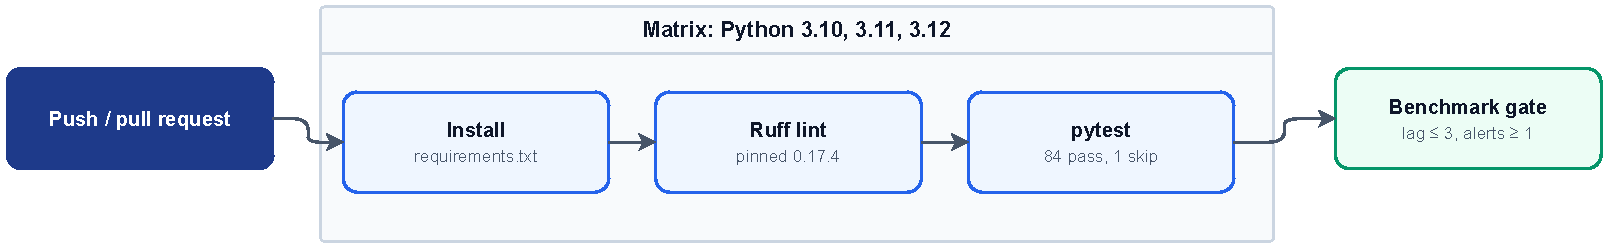
\includegraphics[width=\textwidth]{fig_ci.pdf}
\caption{Continuous-integration pipeline.}
\label{fig:ci}
\end{figure}

\section{Reproducibility}
Every episode is generated from a recorded seed, all models use fixed random states, and bootstrap intervals use fixed generator seeds. A lock file, \texttt{requirements-lock.txt}, records the exact library versions used for the frozen verdicts. The command \texttt{python scripts/reproduce.py} rebuilds whatever is missing and fails if any verdict differs from the saved one. In a clean environment, ten regenerated v8 episodes matched the saved ones to within $4\times10^{-11}$, and the v6, v7 and v8 verdicts were reproduced exactly. The v9 and v10 code is kept on separate branches of the repository because neither was adopted.

\section{Cleaning Up the Prototype}
The original repository contained a Kafka, Celery, Redis and Grafana stack and claims of production readiness that had never been evaluated. We deleted this infrastructure, since it did not help answer the research question, and rewrote the README around the measured results. The legacy FastAPI service, MLflow tracking and PostgreSQL storage were kept as optional components in a separate requirements file.
	% Implementation
%_____________________________________________________________________________________________
% Chapter 6: Results and Discussion
%_____________________________________________________________________________________________

\chapter{Results and Discussion}
\label{ch:results}

All results in this chapter use logistic regression as the monitored model and a label delay of $L=5$ batches with all labels, unless stated otherwise. Intervals are 95\% bootstrap intervals over episodes. Every number comes from a saved verdict or analysis file in \texttt{artifacts/}; the post hoc analyses are marked as such and do not change any verdict.

\section{v6: The Original Design Fails}
\subsection{Benchmark gate}
The v6 protocol required that at least 25\% of shift episodes on development data be harmful, so that the benchmark would contain enough harm to measure. The gate failed at every allowed shift strength (\figref{fig:day2}): only 17--19\% of shifts were harmful, and raising the strength from 1.5 to 4.0 did not change this. Shifts of the more important features were no more often harmful than shifts of the less important ones (0.18 versus 0.17). Because no allowed strength passed and forcing harm (for example, shifting towards misclassified rows) would have made the benchmark partly circular, we proceeded at $\lambda_{max}=1.5$ by a decision recorded before any held-out data were generated. This is reported as a deviation.

\begin{figure}[H]
\centering
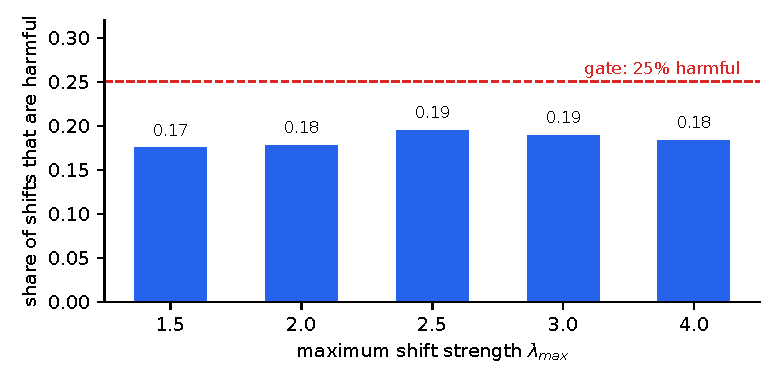
\includegraphics[width=0.75\textwidth]{ch_day2_lambda.pdf}
\caption{Share of development shift episodes that harmed the model, by maximum shift strength. The pre-registered gate required at least 25\%.}
\label{fig:day2}
\end{figure}

\subsection{Pre-registered verdict}
\tabref{tab:v6} shows the verdict on the 5 held-out datasets (53 harmful and 169 harmless shifts). All five hypotheses failed. The learned calibrator warned before the drop on only 22\% of harmful gradual shifts and did not beat waiting for delayed labels. The original DEWS score's higher warning rates on some datasets (\figref{fig:v6ds}) came from alerting almost constantly: on held-out data it raised 36.9 false alerts per 100 clean batches against a budget of 5, while the calibrator raised only 1.2.

\begin{table}[H]
\caption{v6 pre-registered hypotheses on the held-out datasets. Overall verdict: FAILURE.}
\label{tab:v6}
\centering
\small
\begin{tabularx}{\textwidth}{@{}p{5.6cm}Xp{1.25cm}@{}}
\toprule
Hypothesis (target) & Result & Verdict \\
\midrule
H1: T1 on harmful gradual shifts ($\geq$0.60, lead $\geq$2, FA $\leq$5) & 0.22 [0.08, 0.36], lead 12.5, FA 1.2 & Fail \\
H2: T2 gain over waiting for labels ($\geq$0.10, CI $>$0) & 0.83 vs 0.85, $-$0.02 [$-$0.11, 0.08] & Fail \\
H3: harm AUROC ($\geq$0.80); harmless alarms ($\leq$0.10) & 0.59 [0.51, 0.68]; 0.37 & Fail \\
H4: beats the DEWS score ($\geq$4 of 5 datasets) & 2 of 5 & Fail \\
H5: natural streams, T2 gain over labels ($\geq$0) & $-$0.01 [$-$0.08, 0.06] & Fail \\
\bottomrule
\end{tabularx}
\end{table}

\begin{figure}[H]
\centering
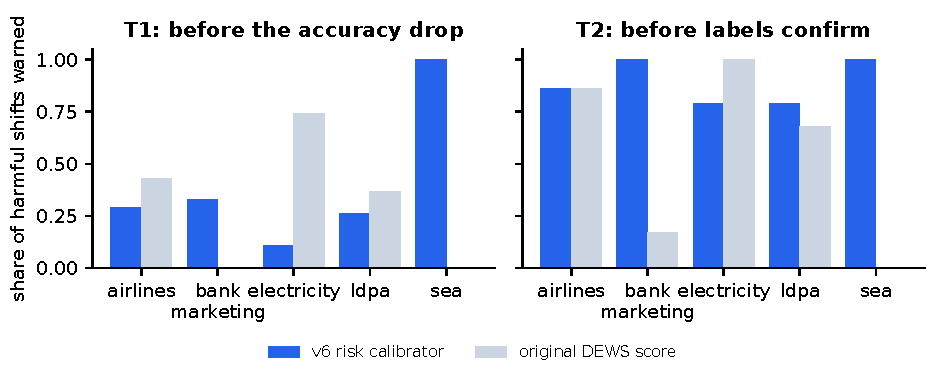
\includegraphics[width=\textwidth]{ch_v6_per_dataset.pdf}
\caption{v6 per held-out dataset: share of harmful shifts warned before the drop (T1) and before labels confirm (T2).}
\label{fig:v6ds}
\end{figure}

\subsection{Secondary settings}
With only 20\% of rows ever labeled (\tabref{tab:scarce}), the gradient-boosting system warned before confirmation more often than the delayed-label trend, but its false alerts exceeded the budget at most delays, and the logistic system stayed below the label trend. We therefore make no claim from these settings.

\begin{table}[H]
\caption{v6 secondary settings with 20\% of labels (held-out): T2 on harmful shifts and false alerts per 100 clean batches.}
\label{tab:scarce}
\centering
\small
\begin{tabular}{@{}lcccc@{}}
\toprule
Model, delay & System T2 & Labels T2 & System FA & Labels FA \\
\midrule
Logistic, $L=0$ & 0.43 & 0.58 & 1.7 & 4.5 \\
Logistic, $L=2$ & 0.38 & 0.57 & 1.0 & 4.0 \\
Logistic, $L=5$ & 0.49 & 0.70 & 1.0 & 5.0 \\
Logistic, $L=10$ & 0.55 & 0.81 & 1.1 & 5.7 \\
Gradient boosting, $L=0$ & 0.64 & 0.48 & 3.9 & 4.0 \\
Gradient boosting, $L=2$ & 0.73 & 0.57 & 5.7 & 5.1 \\
Gradient boosting, $L=5$ & 0.73 & 0.61 & 5.3 & 4.9 \\
Gradient boosting, $L=10$ & 0.82 & 0.80 & 7.7 & 5.9 \\
\bottomrule
\end{tabular}
\end{table}

\section{Why v6 Failed: Thresholds in Raw Units Do Not Transfer}
\figref{fig:transfer} compares, for each method, the false-alert rate on development data (where its threshold was chosen) with the rate on data never used for threshold selection. Scores in dataset-specific units broke the budget by a factor of 3.5--9 (fused DEWS score 4.4 $\rightarrow$ 36.9; mean KS 4.4 $\rightarrow$ 44.6), while the learned calibrator under-alerted (4.6 $\rightarrow$ 1.2). Scores expressed relative to the stream's own normal (drift watch, 2.3 $\rightarrow$ 4.4) or in accuracy points (harm tier, 3.4 $\rightarrow$ 2.8) stayed within the budget on their confirmation data. An ablation of the v6 calibrator confirmed the same mechanism inside the model: removing the raw disagreement levels, which differ widely across datasets, raised its T1 from 0.22 to 0.42. It did not hold everywhere, though. The drift watch broke the budget on natural streams, and the harm tier on the v10 datasets (Section~\ref{sec:followups}).

\begin{figure}[H]
\centering
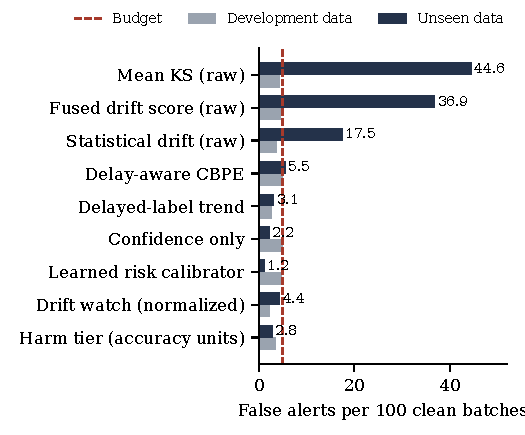
\includegraphics[width=0.8\textwidth]{transfer.pdf}
\caption{False alerts per 100 clean batches with thresholds chosen on development data, on development and on unseen data (v6 held-out data for the v6 methods; v7 and v8 confirmation data for the drift watch and the harm tier). Dashed line: budget of 5.}
\label{fig:transfer}
\end{figure}

\section{v7: The Drift-Watch Tier}
On six fresh datasets (39 harmful gradual shifts) the drift watch warned before the accuracy drop on \textbf{0.87} [0.77, 0.97] of harmful gradual shifts, a median of \textbf{6 batches} ahead, with \textbf{4.4} false alerts per 100 clean batches, and beat the fused DEWS score on 5 of 6 datasets (\tabref{tab:v7}, \figref{fig:v7m}, \figref{fig:v7ds}). Its pre-confirmation warning rate (1.00 against 0.96 for waiting for labels) did not reach the pre-registered gain of 0.10. It also alerted on 96\% of harmless shifts, so it detects drift but cannot tell whether the drift is harmful.

v7 also pre-registered a second tier, a logistic calibrator over the normalised signals. It failed its separation hypothesis (AUROC 0.59, alerts on 53\% of harmless shifts), which motivated the reference-based harm tier of v8.

\begin{table}[H]
\caption{v7 pre-registered hypotheses on six fresh datasets. Overall verdict: PARTIAL SUCCESS.}
\label{tab:v7}
\centering
\small
\begin{tabularx}{\textwidth}{@{}p{5.6cm}Xp{1.25cm}@{}}
\toprule
Hypothesis (target) & Result & Verdict \\
\midrule
C1: WATCH T1 ($\geq$0.60, lead $\geq$2, FA $\leq$5) & 0.87 [0.77, 0.97], lead 6, FA 4.4 & Pass \\
C2: WATCH T2 gain over labels ($\geq$0.10, CI $>$0) & 1.00 vs 0.96, 0.04 [0.00, 0.10] & Fail \\
C3: WARNING separates harm (AUROC $\geq$0.80, harmless $\leq$0.10) & AUROC 0.59; harmless 0.53 & Fail \\
C4: WATCH beats the DEWS score ($\geq$70\% of datasets) & 5 of 6 & Pass \\
C5: natural streams, T2 gain over labels ($\geq$0) & 0.44 vs 0.87, $-$0.43 [$-$0.53, $-$0.32] & Fail \\
\bottomrule
\end{tabularx}
\end{table}

\begin{figure}[H]
\centering
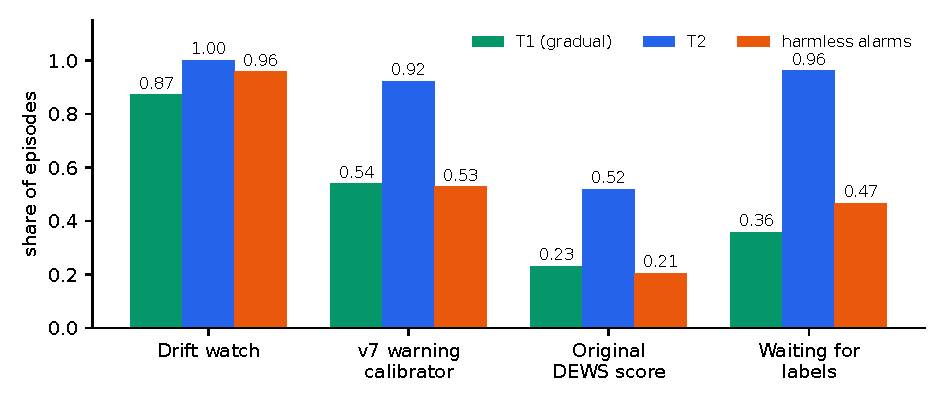
\includegraphics[width=\textwidth]{ch_v7_methods.pdf}
\caption{v7 confirmation data: early warning (T1), pre-confirmation warning (T2) and harmless-shift alarms of each method.}
\label{fig:v7m}
\end{figure}

\begin{figure}[H]
\centering
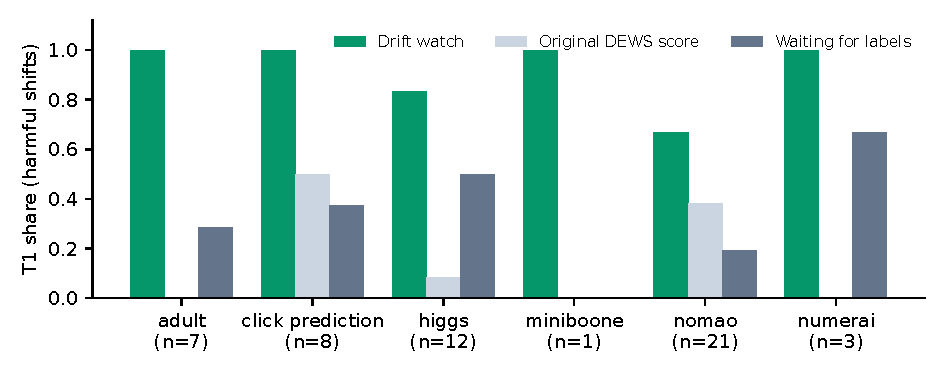
\includegraphics[width=\textwidth]{ch_v7_per_dataset.pdf}
\caption{v7 per confirmation dataset: T1 share of harmful shifts ($n$ = number of harmful shifts).}
\label{fig:v7ds}
\end{figure}

\subsection{Natural streams}
On the 328 natural-stream windows the drift watch failed (T2 0.44 against 0.87 for the label trend) and exceeded the budget (8.0 false alerts per 100 clean batches against 6.3 for the label trend). The data show why. The median degradation began at batch 8, right at the end of the burn-in, and 100 of the 132 events began within 5 batches after it. Accuracy also varied within the burn-in itself (coefficient of variation about 0.12), so the burn-in was not a normal period. Stream normalisation needs a genuinely stable period after deployment.

\section{v8: The Harm Tier}
On five further fresh datasets (64 harmful and 160 harmless shifts) the harm tier cut alarms on harmless shifts from \textbf{0.97} (drift watch) to \textbf{0.34}, while still warning before labels could confirm on 0.83 of harmful shifts and before the drop on 0.76 of harmful gradual shifts, at 2.8 false alerts per 100 clean batches (\tabref{tab:v8}). It separated harmful from harmless shifts with an AUROC of \textbf{0.78} [0.70, 0.86], against 0.59 for the drift watch (gain 0.20 [0.09, 0.30]). It passed two of four hypotheses and missed the AUROC target of 0.80 and the harmless-alarm target of 0.10.

\begin{table}[H]
\caption{v8 pre-registered hypotheses on five fresh datasets. Overall verdict: PARTIAL SUCCESS.}
\label{tab:v8}
\centering
\small
\begin{tabularx}{\textwidth}{@{}p{5.6cm}Xp{1.25cm}@{}}
\toprule
Hypothesis (target) & Result & Verdict \\
\midrule
D1: HARM separates harm (AUROC $\geq$0.80) & 0.78 [0.70, 0.86] & Fail \\
D2: HARM rarely alerts on harmless shifts ($\leq$0.10, FA $\leq$5) & 0.34, FA 2.8 & Fail \\
D3: cuts harmless alarms vs WATCH ($\geq$0.30) with T2 $\geq$0.50 & 0.97 $\rightarrow$ 0.34; T2 0.83 & Pass \\
D4: ranks harm better than WATCH (gain $\geq$0.10, CI $>$0) & 0.78 vs 0.59, gain 0.20 [0.09, 0.30] & Pass \\
\bottomrule
\end{tabularx}
\end{table}

Per dataset (\figref{fig:v8ds}) the harm tier separated harm well on three of the four datasets that produced harmful shifts and was near chance on \emph{kick}; \emph{mv} produced no harmful shift at all.

\begin{figure}[H]
\centering
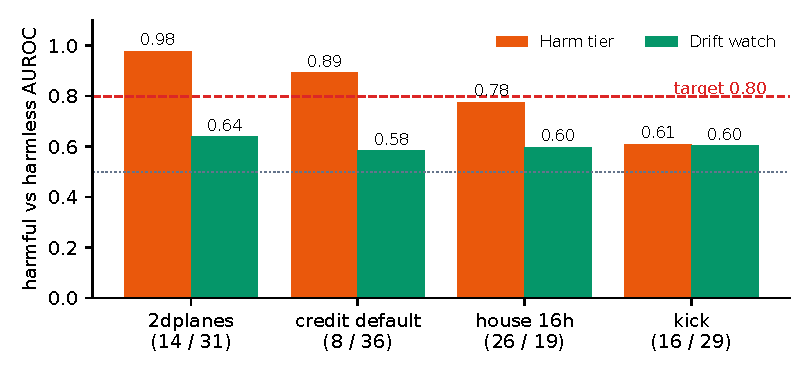
\includegraphics[width=0.85\textwidth]{ch_v8_per_dataset.pdf}
\caption{v8 harmful-versus-harmless AUROC per confirmation dataset (number of harmful / harmless shifts in brackets).}
\label{fig:v8ds}
\end{figure}

\figref{fig:timeline} shows one harmful gradual shift on an unseen dataset. The harm tier first alerts at batch 16, 14 batches before the accuracy event and 20 before delayed labels could confirm it.

\begin{figure}[H]
\centering
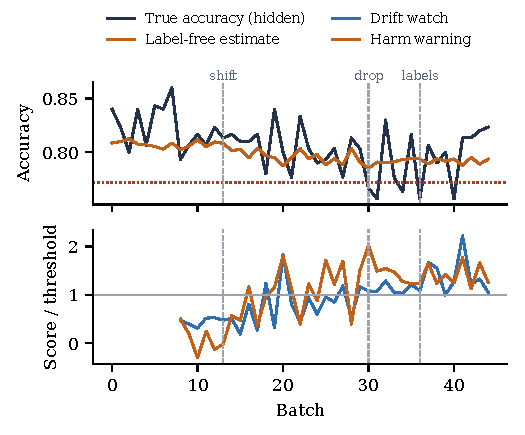
\includegraphics[width=0.8\textwidth]{timeline.pdf}
\caption{A harmful gradual shift on an unseen dataset (credit default, $L=5$). Top: true accuracy (hidden from the monitor) and the label-free estimate; dotted line: 5 points below baseline. Bottom: tier scores divided by their thresholds; above 1 is an alert.}
\label{fig:timeline}
\end{figure}

\section{Same-Data Baselines (Post Hoc)}
To check whether the harm tier is better than simpler label-free estimates, we scored other signals on the v8 confirmation data in exactly the same way (\figref{fig:baselines}). Confidence drop, entropy and delay-aware CBPE reached only 0.56--0.59, and the paired bootstrap interval of the harm tier's advantage over each of them excluded zero. kNN reference accuracy (0.76) and disagreement with models trained on the reference rows (0.73), the other two methods that learn from the labeled reference, were not distinguishable from the harm tier. Confidence drop had reached 0.77 on the v7 data (\tabref{tab:signal_ablation}), so confidence alone is not stable across datasets.

\begin{figure}[H]
\centering
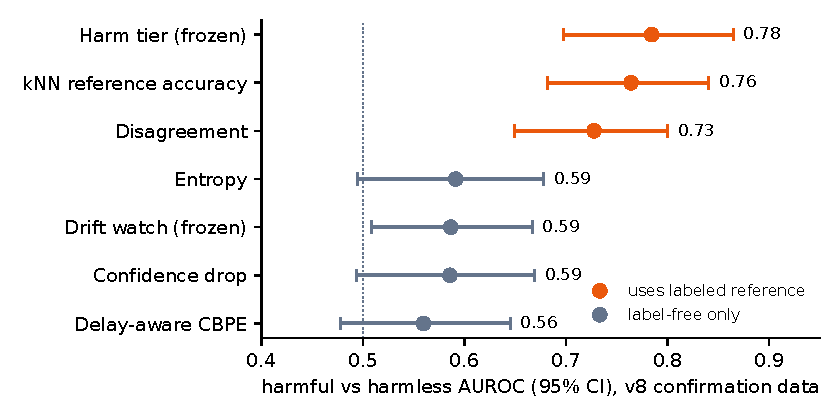
\includegraphics[width=0.8\textwidth]{ch_baselines.pdf}
\caption{Harmful-versus-harmless AUROC of label-free signals on the v8 confirmation data (post hoc), with 95\% bootstrap intervals.}
\label{fig:baselines}
\end{figure}

\section{Why Harmless Shifts Still Alert}
In a post hoc analysis of the v8 confirmation data, streams with no shift at all raised a harm alert in 40\% of episodes and harmless shifts in 34\%, against 88\% for harmful shifts. The harm tier therefore treats harmless shifts like no shift: the remaining alarms are background false alerts that accumulate over about 33 monitored batches. With a per-batch rate of 2.8 per 100, the chance of at least one alert in 33 batches is $1-0.972^{33}\approx 0.6$. Our 10\% target for harmless alarms did not match our own per-batch budget. We noticed this only after the run and left the verdict unchanged.

\figref{fig:operating} shows the full trade-off on the same data. Over most of the range of harmless alarms the harm tier warns on far more harmful shifts than the drift watch. On this data a stricter harm threshold would appear better than the frozen one, but when that idea was frozen and tested on six other datasets (v10, square marker) it warned on only 30\% of harmful shifts. Picking a threshold from this curve after seeing the results would have misled us.

\begin{figure}[H]
\centering
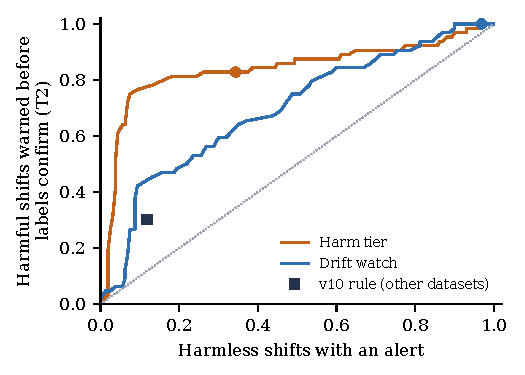
\includegraphics[width=0.75\textwidth]{operating.pdf}
\caption{Post hoc operating curves on the v8 confirmation data; each point is a threshold. Circles: frozen thresholds. Square: the stricter v10 rule, frozen on development data and evaluated on six different datasets.}
\label{fig:operating}
\end{figure}

\section{Pre-Registered Follow-Ups That Failed}
\label{sec:followups}
\textbf{v9: nonlinear harm estimators.} A gradient-boosting domain classifier and an error predictor trained on out-of-fold reference correctness both separated harm worse than the linear estimator on development data (AUROC 0.70 against 0.77). In a post hoc check, ensembles of these estimators, kNN accuracy and confidence (averaging within-dataset ranks) reached at most 0.76. Scored the same way, the linear estimator alone reached 0.75. The 0.80 development gate failed, so no fresh data were used.

\textbf{v10: stricter alerting rules.} Stricter thresholds, exponential smoothing, rolling means, CUSUM, stream-normalised harm scores and gating by the drift watch all reduced harmless alarms at the cost of early warnings. The best rule (a z-scored harm score) passed the development gate, but on six fresh datasets it warned before labels on only 0.30 of harmful shifts against a required 0.50, while reducing harmless alarms to 0.12. Neither v9 nor v10 was adopted.

On the same six v10 datasets the frozen v8 rule warned before labels on 0.74 of harmful shifts but alerted on 58\% of harmless shifts and raised \textbf{12.7} false alerts per 100 clean batches, more than twice the budget. Its calibration therefore did not hold on every new dataset. \figref{fig:tradeoff} places these operating points side by side.

\begin{figure}[H]
\centering
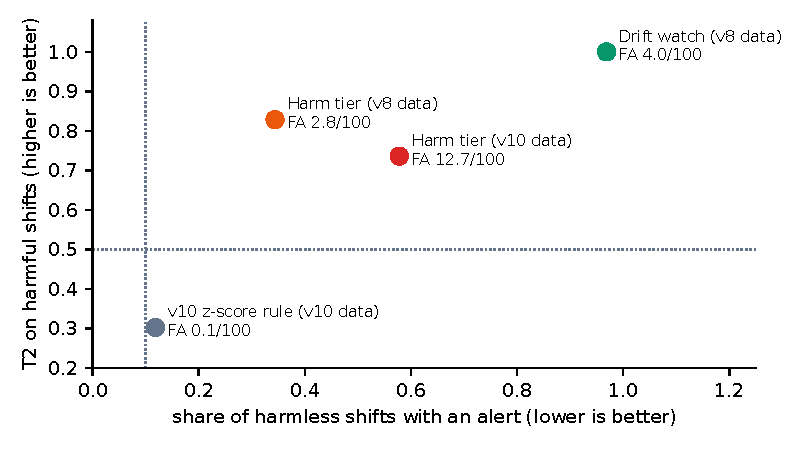
\includegraphics[width=0.78\textwidth]{ch_tradeoff.pdf}
\caption{Harmless-shift alarms against pre-confirmation warnings for the frozen tiers and the v10 rule; FA = false alerts per 100 clean batches.}
\label{fig:tradeoff}
\end{figure}

\section{Ablations}
\subsection{Two families of signals}
Using each normalised signal alone as the drift watch on the v7 confirmation data (\tabref{tab:signal_ablation}, \figref{fig:families}) shows two families with opposite strengths. Input-shift signals warned early on 79--90\% of harmful gradual shifts but could not tell harm from harmlessness (AUROC about 0.5). Model-behaviour signals were harm-aware (AUROC 0.72--0.77) but warned later. Removing any single signal from the drift watch changed little, so no signal is a single point of failure.

\begin{table}[H]
\caption{Each normalised signal used alone (v7 confirmation data, post hoc).}
\label{tab:signal_ablation}
\centering
\small
\begin{tabular}{@{}llccc@{}}
\toprule
Family & Signal & T1 & Harmless alarms & AUROC \\
\midrule
Input shift & fused DEWS score & 0.90 & 0.95 & 0.52 \\
 & mean KS & 0.90 & 0.95 & 0.53 \\
 & relevance-weighted shift & 0.79 & 0.92 & 0.51 \\
 & positive-rate shift & 0.79 & 0.73 & 0.54 \\
Model behaviour & disagreement & 0.49 & 0.42 & 0.72 \\
 & confidence drop & 0.46 & 0.24 & 0.77 \\
 & entropy & 0.41 & 0.25 & 0.75 \\
\midrule
All 7 (drift watch) & & 0.87 & 0.96 & 0.51 \\
\bottomrule
\end{tabular}
\end{table}

\begin{figure}[H]
\centering
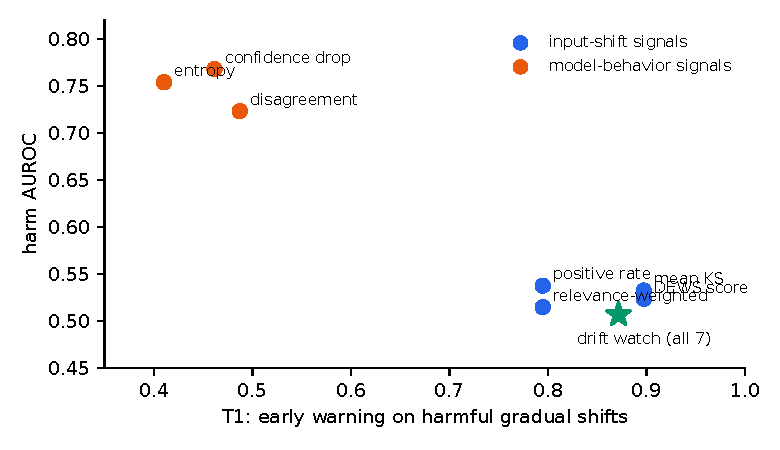
\includegraphics[width=0.72\textwidth]{ch_signal_families.pdf}
\caption{Early warning versus harm separation of each signal used alone (v7 confirmation data).}
\label{fig:families}
\end{figure}

\subsection{Which harm estimator}
All reference-based estimators reached about the same separation on the v8 confirmation data (AUROC 0.76--0.78), far above every drift signal (\tabref{tab:harm_est}). The gain comes from using the labeled reference, not from the particular estimator. The variants trade sensitivity for quietness: nearest-neighbour accuracy is the quietest but warns less.

\begin{table}[H]
\caption{Harm-estimator variants on the v8 confirmation data (thresholds by the separation rule).}
\label{tab:harm_est}
\centering
\small
\begin{tabular}{@{}lccccc@{}}
\toprule
Estimator & T1 & T2 & FA & Harmless alarms & AUROC \\
\midrule
Importance-weighted (frozen) & 0.76 & 0.83 & 2.8 & 0.34 & 0.78 \\
Nearest-neighbour & 0.49 & 0.70 & 0.2 & 0.17 & 0.76 \\
Average of both & 0.71 & 0.83 & 1.0 & 0.29 & 0.78 \\
\bottomrule
\end{tabular}
\end{table}

\subsection{Why most shifts are harmless}
In every data group about 70--80\% of shifts did not harm the model (\figref{fig:harmrates}). Whether harm occurred was barely related to the importance of the shifted feature (the difference appeared only in the v8 group) and not related to the model's baseline accuracy. Harm depends on whether the shift moves data into regions where this particular model is wrong. That explains why feature-importance weighting (v5) failed and why reference-based estimation (v8) was the first approach to separate harmful from harmless shifts.

\begin{figure}[H]
\centering
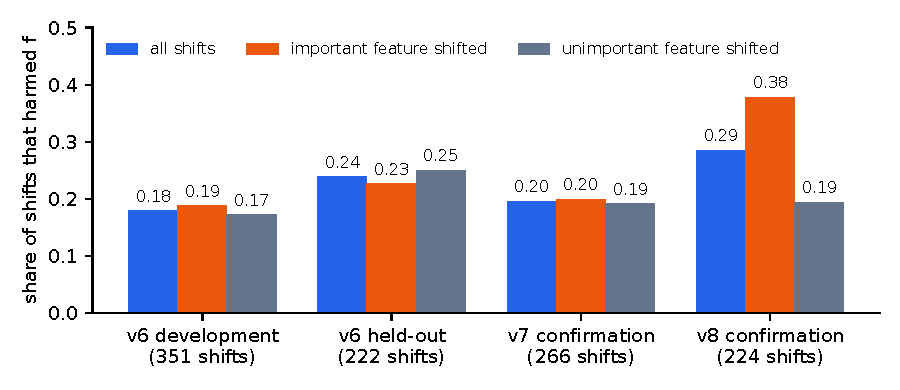
\includegraphics[width=0.9\textwidth]{ch_harm_rates.pdf}
\caption{Share of shift episodes that harmed the model, by data group and by importance of the shifted feature.}
\label{fig:harmrates}
\end{figure}

\section{Discussion}
\subsection{Lessons}
\begin{enumerate}
\item \textbf{Comparable units made thresholds transfer.} The step from v6 to v7 did not need a better model, since the drift watch is simpler than the v6 calibrator; what changed was the scale of the signals. It did not solve everything: the harm rule still broke the budget on the v10 datasets, and the drift watch did on natural streams. Alert thresholds tuned on historical data should be validated on data from other sources before deployment.
\item \textbf{Separate a sensitive drift tier from a specific harm tier.} Input-shift signals are good for early notice; model-behaviour and reference-based signals are needed to judge harm.
\item \textbf{Keep a labeled reference sample.} In our data, only methods that used it separated harm consistently across datasets.
\item \textbf{Make per-episode targets consistent with per-batch budgets.} A 2.8\% per-batch false-alert rate already implies about a 60\% chance of an alarm over 33 batches.
\item \textbf{Several ideas failed on new data.} Online updating (v2), relevance weighting (v5), nonlinear estimators (v9) and stricter rules (v10) all looked useful during development and did not hold up.
\end{enumerate}

\subsection{Threats to validity}
The v7 and v8 designs were motivated by the v6 failure, so they are informed by data we had already seen; we mitigated this by confirming each on datasets downloaded only after its design was frozen, but the sequence of experiments was not planned in advance. The 13 v6 datasets had been explored in v1--v5, so the v6 held-out results are not fully out of sample. Harmful-shift counts per confirmation group (52--64; 39 gradual in v7) give confidence intervals of roughly $\pm$0.1. The event rule (two batches at least 5 points below baseline) and the horizon are conventional choices that we did not vary. Pre-registration was internal (git commits), not on a public registry.

\subsection{Limitations}
Shifts are constructed by re-sampling real rows, which preserves $P(y\mid x)$ and thus favours covariate-shift methods; changes in the label relationship are invisible to every label-free signal until labels arrive. The confirmed model is logistic regression only; the burn-in assumes a stable start, which failed on natural streams; the setting is binary tabular data with 20 features and batches of 300 rows; and the per-dataset numbers of harmful shifts are small, so intervals are wide. The harm tier trains a domain classifier on every batch, and its run-time cost was not measured systematically.
	% Results and discussion
%_____________________________________________________________________________________________
% Chapter 7: Conclusion and Future Work
%_____________________________________________________________________________________________

\chapter{Conclusion and Future Work}
\label{ch:conclusion}

\section{Conclusion}
This project set out to build an ML model drift early-warning system that warns about degradation, not merely drift, before delayed labels can confirm it. We built a benchmark that re-samples real tabular data so that whether a shift harms the model is measured from true labels, and we evaluated ten versions of the system, five of them with pre-registered hypotheses, frozen thresholds and one-time runs on unseen datasets.

The results are mixed, and we report them as they are:
\begin{itemize}
\item The original design, a learned risk calibrator over raw drift scores, failed all its hypotheses, because thresholds in dataset-specific units did not transfer across datasets.
\item A stream-normalised \textbf{drift watch} gave early warning of harmful drift within its false-alert budget on benchmark streams: on six fresh datasets it warned before the accuracy drop on 87\% of harmful gradual shifts, a median of six batches ahead. It cannot tell harmful from harmless drift, and it failed on natural streams where drift had begun before monitoring.
\item An importance-weighted \textbf{harm tier} reduced alarms on harmless shifts from 97\% to 34\% and separated harmful from harmless shifts with an AUROC of 0.78, short of the 0.80 target but above confidence-based baselines on the same data. On a later set of datasets its false-alert rate exceeded the budget.
\item Nonlinear estimators, ensembles and stricter alerting rules did not improve on it.
\end{itemize}
Without labels, our best estimator separated harmful from harmless shifts only partly, and it needed a labeled reference set. The practical lessons are to express alert scores in units that are comparable across streams, to validate thresholds on data from other sources, to separate a sensitive drift tier from a specific harm tier, and to keep a labeled reference sample.

Beyond the research findings, the project delivers a working and reproducible product: the monitoring library, frozen configurations and verdict scripts, a dashboard that replays monitored streams with delayed labels, 85 unit tests with continuous integration, and a research paper.

\section{Future Work}
\begin{enumerate}
\item \textbf{Better burn-in handling.} Detect whether the burn-in itself is stable, or use a reference period chosen with labels, so that stream normalisation also works when drift has begun before monitoring.
\item \textbf{Calibrated harm alerting.} Control the false-alert rate over a whole monitoring period (for example with sequential testing) instead of per batch, so that per-episode alarm targets become achievable.
\item \textbf{Richer density-ratio estimation.} Combine importance weighting with uncertainty estimates, and test other models than logistic regression as the monitored model.
\item \textbf{Label changes.} Use the few labels that arrive early (partial labeling) to detect changes in $P(Y\mid X)$, which no input-only signal can see.
\item \textbf{More data types.} Extend the benchmark to multi-class, text and image data, and to real temporal streams with documented drift.
\item \textbf{Deployment.} Package the two tiers as a service that reads batches from a production pipeline, with the dashboard as its operator view.
\item \textbf{Public pre-registration.} Register future experiments on a public registry before running them.
\end{enumerate}
	% Conclusion and future work

\appendix
%_____________________________________________________________________________________________
% Appendices
%_____________________________________________________________________________________________

\chapter{Pre-Registered Hypotheses}
\label{app:hyp}
Every hypothesis below was committed to the repository, with its pass rule, before the data that judged it were downloaded. The overall verdict rule of each experiment was fixed at the same time.

\begin{longtable}{@{}p{1.0cm}p{6.2cm}p{5.2cm}p{1.5cm}@{}}
\toprule
ID & Claim & Pass rule & Result \\
\midrule
\endhead
\multicolumn{4}{@{}l}{\textbf{v6} (held-out datasets; success if H1 and H3 pass)} \\
H1 & Predictive warning for gradual harmful shifts & T1 $\geq$ 0.60, median lead $\geq$ 2, FA $\leq$ 5 & Fail \\
H2 & Earlier than waiting for labels & T2 gain $\geq$ 0.10, paired CI $>$ 0 & Fail \\
H3 & Separates harmful from harmless shifts & AUROC $\geq$ 0.80, harmless $\leq$ 0.10 & Fail \\
H4 & Beats the original DEWS score & higher T1 and T2 on $\geq$ 4 of 5 datasets & Fail \\
H5 & Carries over to natural streams & T2 gain over labels $\geq$ 0 & Fail \\
\midrule
\multicolumn{4}{@{}l}{\textbf{v7} (six fresh datasets; success if C1 and C3 pass)} \\
C1 & WATCH warns before the accuracy drop & T1 $\geq$ 0.60, lead $\geq$ 2, FA $\leq$ 5 & Pass \\
C2 & WATCH warns before labels, better than labels & gain $\geq$ 0.10, CI $>$ 0 & Fail \\
C3 & WARNING separates harmful from harmless & AUROC $\geq$ 0.80, harmless $\leq$ 0.10 & Fail \\
C4 & WATCH beats the DEWS score & higher T1 and T2 on $\geq$ 70\% of datasets & Pass \\
C5 & WATCH carries over to natural streams & T2 gain over labels $\geq$ 0 & Fail \\
\midrule
\multicolumn{4}{@{}l}{\textbf{v8} (five fresh datasets; success if D1 and D2 pass)} \\
D1 & HARM separates harmful from harmless & AUROC $\geq$ 0.80 & Fail \\
D2 & HARM rarely alerts on harmless shifts & harmless $\leq$ 0.10, FA $\leq$ 5 & Fail \\
D3 & HARM cuts harmless alarms vs WATCH while warning & drop $\geq$ 0.30, T2 $\geq$ 0.50, FA $\leq$ 5 & Pass \\
D4 & HARM ranks harm better than WATCH & gain $\geq$ 0.10, CI $>$ 0 & Pass \\
\midrule
\multicolumn{4}{@{}l}{\textbf{v9} (development gate)} \\
G9 & A nonlinear estimator reaches the target & development AUROC $\geq$ 0.80 & Fail \\
\midrule
\multicolumn{4}{@{}l}{\textbf{v10} (six fresh datasets; all three required)} \\
E1 & Few harmless alarms & harmless $\leq$ 0.15 & Pass \\
E2 & Still warns before labels & T2 $\geq$ 0.50 & Fail \\
E3 & Within the false-alert budget & FA $\leq$ 5 & Pass \\
\bottomrule
\end{longtable}

\chapter{Datasets}
\label{app:data}
All datasets were obtained from OpenML~\cite{vanschoren2014openml}. For multi-class targets the majority class is used against the rest; the first 20 non-constant features are used.

\begin{longtable}{@{}p{3.2cm}p{11.6cm}@{}}
\toprule
Group & Datasets (OpenML IDs where recorded in the protocol) \\
\midrule
\endhead
v6 development & covertype, CovPokElec, Hyperplane, KDDCup99, LED, poker-hand, run-or-walk, vehicle-SensIT \\
v6 held-out & airlines, bank-marketing, electricity, ldpa, SEA (drawn with \texttt{default\_rng(2026)}) \\
v7 confirmation & adult (1590), MiniBooNE (41150), higgs (23512), nomao (1486), numerai28.6 (23517), Click\_prediction\_small (1220) \\
v8 confirmation & default-of-credit-card-clients (42477), kick (41162), house\_16H (821), 2dplanes (727), mv (881); albert (41147) could not be downloaded and was dropped before any episode was built \\
v10 confirmation & road-safety (42803), Diabetes130US (4541), jannis (41168), rl (41160), fried (901), jungle\_chess (41027) \\
Natural streams & 328 non-overlapping row-order windows of the 13 v6 datasets (from studies v2--v4) \\
\bottomrule
\end{longtable}

\noindent\textbf{Recorded deviations.} MiniBooNE (v7) and rl (v10) store their rows sorted by class, so no contiguous block contains both classes; each was shuffled once with a fixed seed before any confirmation episode was built.

\chapter{Reproducing the Results}
\label{app:repro}
\section{Environment}
{\small
\begin{verbatim}
python -m venv .venv
.venv\Scripts\activate          # Linux: source .venv/bin/activate
pip install -r requirements-lock.txt
\end{verbatim}
}

\section{Verdicts, ablations and post hoc analyses}
{\small
\begin{verbatim}
python scripts/reproduce.py --dry-run   # show the plan
python scripts/reproduce.py             # rebuild and verify
python scripts/run_ablations.py
python scripts/run_posthoc.py
\end{verbatim}
}

\section{Dashboard, tests, figures}
{\small
\begin{verbatim}
streamlit run streamlit_app.py
pytest -q
python scripts/make_paper_figures.py
python report/figures/make_report_charts.py
python report/figures/drawio/build_diagrams.py
python report/figures/drawio/export_drawio.py
\end{verbatim}
}

\section{Frozen files}
\begin{table}[H]
\centering
\small
\begin{tabular}{@{}lll@{}}
\toprule
Experiment & File & SHA-256 (prefix) \\
\midrule
v6 & \texttt{artifacts/v6/frozen\_choices.json} & 93019702\ldots e4ad \\
v6 & \texttt{artifacts/v6/frozen\_calibrators.pkl} & 93f58147\ldots 409e \\
v7 & \texttt{artifacts/v7/frozen\_v7.json} & 4a9ab970cb58fad9 \\
v7 & \texttt{artifacts/v7/frozen\_v7\_calibrator.pkl} & dab467db1cc2045e \\
v8 & \texttt{artifacts/v8/frozen\_v8.json} & b8005ca95d70cc4f \\
v10 & \texttt{artifacts/v10/frozen\_v10.json} & c30860f3adda1561 \\
\bottomrule
\end{tabular}
\end{table}


\bibliographystyle{plain}
\bibliography{coep_compit_report}
\addcontentsline{toc}{chapter}{Bibliography}
%_____________________________________________________________________________________________
\end{document}			% End of Report
